\documentclass{beamer}

\mode<presentation>
{
  \useinnertheme{rounded}
  \useoutertheme{infolines}
  \usecolortheme{wolverine}
  \setbeamercovered{transparent}
}

\usepackage[english]{babel}

\usepackage[latin1]{inputenc}

\usepackage{avant}
\usepackage[T1]{fontenc}

\usepackage{multimedia}

\title[Simulation of Al Foam]
{Numerical simulation of the dynamic compression of a 6061-T6 aluminum
metallic foam}

\author[B. Banerjee, A. Bhawalkar]{Biswajit Banerjee and Anup Bhawalkar}
\institute[Univ. of Utah]
{Center for the Simulation of Accidental Fires and Explosions\\
  University of Utah}

\date[WCCM VII - 2006]
{7th World Conference on Computational Mechanics, 2006}

\subject{Foam Compression}

%\AtBeginSubsection[]
%{
%  \begin{frame}<beamer>
%    \frametitle{Outline}
%    \tableofcontents[currentsection,currentsubsection]
%  \end{frame}
%}

\definecolor{red}{rgb}{1,0,0}
\definecolor{green}{rgb}{0,1,0}
\definecolor{blue}{rgb}{0,0,1}
\definecolor{Red}{rgb}{0.8666,0.03137,0.02352}
\definecolor{Blue}{rgb}{0.00784,0.67059,0.91764}
\definecolor{Darkgreen}{rgb}{0,0.68235,0}
\definecolor{Green}{rgb}{0,0.8,0}
\definecolor{Bl}{rgb}{0,0.2,0.91764}
\definecolor{Royalblue}{rgb}{0,0.2,0.91764}
\definecolor{Brickred}{rgb}{0.644541,0.164065,0.164065}
\definecolor{Brown}{rgb}{0.6,0.4,0.4}
\definecolor{Orange}{rgb}{1,0.647059,0}
\definecolor{Indigo}{rgb}{0.746105,0,0.996109}
\definecolor{Violet}{rgb}{0.308598,0.183597,0.308598}
\definecolor{Lightgrey}{rgb}{0.762951,0.762951,0.762951}
\definecolor{Darkgrey}{rgb}{0.503548,0.503548,0.503548}
\definecolor{Pink}{rgb}{1,0.6,0.6}
\definecolor{MyLightMagenta}{cmyk}{0.1,0.8,0,0.1}
\definecolor{MyDarkBlue}{rgb}{0,0.08,0.45}
\newcommand{\Red}{\color{Brickred}}
\newcommand{\Blue}{\color{Royalblue}}
\newcommand{\Green}{\color{Darkgreen}}
\newcommand{\Violet}{\color{Violet}}
\providecommand{\abs}[1]{\lvert#1\rvert}
\providecommand{\norm}[1]{\lVert#1\rVert}
\newcommand{\erf}{\text{erf}}
\newcommand{\Ep}{\ensuremath{\epsilon_p}}
\newcommand{\Epi}{\ensuremath{\epsilon_{pi}}}
%\newcommand{\Epdot}[1]{\ensuremath{\dot{\epsilon}_{p#1}}}
\newcommand{\Epdot}[1]{\ensuremath{\dot{\epsilon}_{#1}}}
\newcommand{\Xidot}{\ensuremath{\dot{\xi}}}
\newcommand{\Sa}{\ensuremath{\sigma_a}}
\newcommand{\Shi}{\ensuremath{\hat\sigma_i}}
\newcommand{\She}{\ensuremath{\hat\sigma_e}}
\newcommand{\Gi}{\ensuremath{g_{0i}}}
\newcommand{\Ge}{\ensuremath{g_{0e}}}
\newcommand{\Ei}{\ensuremath{\dot\epsilon_{0i}}}
\newcommand{\Ee}{\ensuremath{\dot\epsilon_{0e}}}
\newcommand{\En}{\ensuremath{\epsilon_{n}}}
\newcommand{\Pci}{\ensuremath{p_{i}}}
\newcommand{\Pce}{\ensuremath{p_{e}}}
\newcommand{\Qci}{\ensuremath{q_{i}}}
\newcommand{\Qce}{\ensuremath{q_{e}}}
\newcommand{\To}{\ensuremath{\theta_{0}}}
\newcommand{\TIV}{\ensuremath{\theta_{IV}}}
\newcommand{\Ses}{\ensuremath{\hat\sigma_{es0}}}
\newcommand{\Ges}{\ensuremath{g_{0es}}}
\newcommand{\Ees}{\ensuremath{\dot\epsilon_{es0}}}
\newcommand{\Ve}{\ensuremath{\varepsilon}}
\newcommand{\BH}[1]{\ensuremath{\hat{\boldsymbol{#1}}}}
\newcommand{\BTx}{\ensuremath{\tilde{\boldsymbol{x}}}}
\newcommand{\Beh}{\ensuremath{\hat{\boldsymbol{e}}}}
\newcommand{\BHex}{\ensuremath{\hat{\boldsymbol{e}}_1}}
\newcommand{\BHey}{\ensuremath{\hat{\boldsymbol{e}}_2}}
\newcommand{\BHez}{\ensuremath{\hat{\boldsymbol{e}}_3}}
\newcommand{\BHn}[1]{\ensuremath{\hat{\boldsymbol{n}}_{#1}}}
\newcommand{\BHe}[1]{\ensuremath{\hat{\boldsymbol{e}}_{#1}}}
\newcommand{\BHg}[1]{\ensuremath{\hat{\boldsymbol{g}}_{#1}}}
\newcommand{\BHG}[1]{\ensuremath{\hat{\boldsymbol{G}}_{#1}}}
\newcommand{\Bnhat}{\ensuremath{\hat{\boldsymbol{n}}}}
\newcommand{\That}{\ensuremath{\hat{T}}}
\newcommand{\Mu}{\ensuremath{\left[u\right]}}
\newcommand{\Mv}{\ensuremath{\left[v\right]}}
\newcommand{\MA}{\ensuremath{\left[A\right]}}
\newcommand{\MC}{\ensuremath{\left[C\right]}}
\newcommand{\MD}{\ensuremath{\left[D\right]}}
\newcommand{\ML}{\ensuremath{\left[L\right]}}
\newcommand{\MT}{\ensuremath{\left[T\right]}}
\newcommand{\Msig}{\ensuremath{\left[\boldsymbol{\sigma}\right]}}
\newcommand{\Meps}{\ensuremath{\left[\boldsymbol{\varepsilon}\right]}}
\newcommand{\Ex}{\ensuremath{\boldsymbol{e}_1}}
\newcommand{\Ey}{\ensuremath{\boldsymbol{e}_2}}
\newcommand{\Ez}{\ensuremath{\boldsymbol{e}_3}}
\newcommand{\Exp}{\ensuremath{\boldsymbol{e}^{'}_1}}
\newcommand{\Eyp}{\ensuremath{\boldsymbol{e}^{'}_2}}
\newcommand{\Ezp}{\ensuremath{\boldsymbol{e}^{'}_3}}
\newcommand{\Epsxx}{\ensuremath{\varepsilon_{11}}}
\newcommand{\Epsyy}{\ensuremath{\varepsilon_{22}}}
\newcommand{\Epszz}{\ensuremath{\varepsilon_{33}}}
\newcommand{\Epsyz}{\ensuremath{\varepsilon_{23}}}
\newcommand{\Epszx}{\ensuremath{\varepsilon_{31}}}
\newcommand{\Epsxy}{\ensuremath{\varepsilon_{12}}}
\newcommand{\Sigxx}{\ensuremath{\sigma_{11}}}
\newcommand{\Sigyy}{\ensuremath{\sigma_{22}}}
\newcommand{\Sigzz}{\ensuremath{\sigma_{33}}}
\newcommand{\Sigyz}{\ensuremath{\sigma_{23}}}
\newcommand{\Sigzx}{\ensuremath{\sigma_{31}}}
\newcommand{\Sigxy}{\ensuremath{\sigma_{12}}}
\newcommand{\X}{\ensuremath{X_1}}
\newcommand{\Y}{\ensuremath{X_2}}
\newcommand{\Z}{\ensuremath{X_3}}
\newcommand{\Bchi}{\ensuremath{\boldsymbol{\chi}}}
\newcommand{\Beps}{\ensuremath{\boldsymbol{\varepsilon}}}
\newcommand{\Bbeps}{\ensuremath{\bar{\boldsymbol{\varepsilon}}}}
\newcommand{\Bnabla}{\ensuremath{\boldsymbol{\nabla}}}
\newcommand{\Bomega}{\ensuremath{\boldsymbol{\omega}}}
\newcommand{\Bsig}{\ensuremath{\boldsymbol{\sigma}}}
\newcommand{\Bvarphi}{\ensuremath{\boldsymbol{\varphi}}}
\newcommand{\Blambda}{\ensuremath{\boldsymbol{\lambda}}}
\newcommand{\Bmu}{\ensuremath{\boldsymbol{\mu}}}
\newcommand{\Beta}{\ensuremath{\boldsymbol{\eta}}}
\newcommand{\Bone}{\ensuremath{\boldsymbol{1}}}
\newcommand{\Bzero}{\ensuremath{\boldsymbol{0}}}
\newcommand{\Ba}{\ensuremath{\boldsymbol{a}}}
\newcommand{\Bb}{\ensuremath{\boldsymbol{b}}}
\newcommand{\Bc}{\ensuremath{\boldsymbol{c}}}
\newcommand{\Bd}{\ensuremath{\boldsymbol{d}}}
\newcommand{\Be}{\ensuremath{\boldsymbol{e}}}
\newcommand{\Bf}{\ensuremath{\boldsymbol{f}}}
\newcommand{\Bg}{\ensuremath{\boldsymbol{g}}}
\newcommand{\Bm}{\ensuremath{\boldsymbol{m}}}
\newcommand{\Bn}{\ensuremath{\boldsymbol{n}}}
\newcommand{\Bp}{\ensuremath{\boldsymbol{p}}}
\newcommand{\Bq}{\ensuremath{\boldsymbol{q}}}
\newcommand{\Br}{\ensuremath{\boldsymbol{r}}}
\newcommand{\Bs}{\ensuremath{\boldsymbol{s}}}
\newcommand{\Bt}{\ensuremath{\boldsymbol{t}}}
\newcommand{\Bu}{\ensuremath{\boldsymbol{u}}}
\newcommand{\Bv}{\ensuremath{\boldsymbol{v}}}
\newcommand{\Bw}{\ensuremath{\boldsymbol{w}}}
\newcommand{\Bx}{\ensuremath{\boldsymbol{x}}}
\newcommand{\BA}{\ensuremath{\boldsymbol{A}}}
\newcommand{\BC}{\ensuremath{\boldsymbol{C}}}
\newcommand{\BD}{\ensuremath{\boldsymbol{D}}}
\newcommand{\BE}{\ensuremath{\boldsymbol{E}}}
\newcommand{\BF}{\ensuremath{\boldsymbol{F}}}
\newcommand{\BG}{\ensuremath{\boldsymbol{G}}}
\newcommand{\BI}{\ensuremath{\boldsymbol{I}}}
\newcommand{\BM}{\ensuremath{\boldsymbol{M}}}
\newcommand{\BP}{\ensuremath{\boldsymbol{P}}}
\newcommand{\BQ}{\ensuremath{\boldsymbol{Q}}}
\newcommand{\BT}{\ensuremath{\boldsymbol{T}}}
\newcommand{\BW}{\ensuremath{\boldsymbol{W}}}
\newcommand{\BX}{\ensuremath{\boldsymbol{X}}}
\newcommand{\BY}{\ensuremath{\boldsymbol{Y}}}
\newcommand{\Tor}{\ensuremath{\text{,~or}}}
\newcommand{\Tr}{\ensuremath{\text{~tr}}}
\newcommand{\Dev}{\ensuremath{\text{~dev}}}
\newcommand{\Tint}{\ensuremath{\text{int}}}
\newcommand{\Text}{\ensuremath{\text{ext}}}
\newcommand{\Tg}{\ensuremath{\text{g}}}
\newcommand{\Tp}{\ensuremath{\text{p}}}

\newcommand{\Half}{\ensuremath{\frac{1}{2}}}
\newcommand{\SThr}{\ensuremath{\sqrt{3}}}
\newcommand{\STT}{\ensuremath{\frac{\sqrt{3}}{2}}}
\newcommand{\Third}{\ensuremath{\frac{1}{3}}}
\newcommand{\Bcross}[2]{\ensuremath{#1\boldsymbol{\times}#2}}
\newcommand{\Bdot}[2]{\ensuremath{#1\bullet#2}}
\newcommand{\Bdual}[2]{\ensuremath{#1\boldsymbol{\otimes}#2}}
\newcommand{\Grad}[1]{\ensuremath{\Bnabla #1}}
\newcommand{\Lap}[1]{\ensuremath{\nabla^2 #1}}
\newcommand{\Biharm}[1]{\ensuremath{\nabla^4 #1}}
\newcommand{\Div}[1]{\ensuremath{\Bdot{\Bnabla}{#1}}}
\newcommand{\Curl}[1]{\ensuremath{\Bcross{\Bnabla}{#1}}}
\newcommand{\Gradu}{\ensuremath{\Grad{\Bu}}}
\newcommand{\Divu}{\ensuremath{\Div{\Bu}}}
\newcommand{\Curlu}{\ensuremath{\Curl{\Bu}}}
\newcommand{\Dualn}{\ensuremath{\Bdual{\Bn}{\Bn}}}
\newcommand{\Over}[1]{\ensuremath{\frac{1}{#1}}}
\newcommand{\Partial}[2]{\ensuremath{\frac{\partial #1}{\partial #2}}}
\newcommand{\PPartial}[2]{\ensuremath{\frac{\partial^2 #1}{\partial #2^2}}}
\newcommand{\PPartialA}[3]{\ensuremath{\frac{\partial^2 #1}{\partial #2\partial#3}}}
\newcommand{\FPartial}[2]{\ensuremath{\frac{\partial^4 #1}{\partial #2^4}}}
\newcommand{\FPartialA}[3]{\ensuremath{\frac{\partial^4 #1}{\partial #2^2
         \partial #3^2}}}



\begin{document}

  \begin{frame}
    \titlepage
  \end{frame}

  \begin{frame}
    \frametitle{Outline}
    \tableofcontents
  \end{frame}

  \section{Motivation}

    \begin{frame}
      \frametitle{Why Aluminum Foams?}
      \begin{columns}[c]
        \begin{column}{4cm}
          \scalebox{0.2}{\includegraphics{FIGS/AlFoamMicrostructure.jpg}} \\
          {\tiny (Physics Today (2002), {\bf 55}, 37-42) }
        \end{column}
        \begin{column}{6cm}
          \begin{itemize}[<+-| alert@+>]
            \item Low weight to volume ratio.
            \item High weight to specific mechanical stiffness.  
            \item Used for:
              \begin{itemize}
                \item High-capacity impact absorption.
                \item Acoustic and thermal control.
              \end{itemize}
          \end{itemize}
        \end{column}
      \end{columns}
    \end{frame}

    \begin{frame}
      \frametitle{Challenges}
      \begin{itemize}[<+-| alert@+>]
        \item Determination of dynamic structure/property relations.\\
              \vspace{12pt}
        \item Homogenization of nonlinear dynamic processes
              is nontrivial.\\
              \vspace{12pt}
        \item We would like to determine whether gases inside
              closed-cell foams have a significant effect. 
      \end{itemize}
    \end{frame}

    \subsection{Previous Work}
    \begin{frame}
      \frametitle{Previous Work: Models}
      \begin{itemize}[<+-| alert@+>]
        \item Gibson and Ashby (1997):
          \begin{itemize}
            \item Detailed exposition of structure-property relations
              in cellular solids.  
            \item Simplified microstructures.
          \end{itemize}
        \item Ashby et al. (2000):
          \begin{itemize}
            \item A design guide for metal foams.
            \item A small-strain plasticity model was presented.
          \end{itemize}
        \item Deshpande and Fleck (2000):
          \begin{itemize}
            \item Detailed study of yield surfaces.
            \item Improved plasticity model for small strains.
          \end{itemize}
        \item Schmidt (2004):
          \begin{itemize}
            \item Model of elastic-plastic anisotropy in metal foams.
            \item Large strain effects included.
          \end{itemize}
        \item Benke and Weichert (2005):
          \begin{itemize}
            \item Model incorporates effect of fluid pressure.
          \end{itemize}
      \end{itemize}
    \end{frame}

    \begin{frame}
      \frametitle{Previous Work: Experiments and Simulations}
      \begin{itemize}[<+-| alert@+>]
        \item Deshpande and Fleck (2000), Paul and Ramamurty (2000),
              Danneman and Lankford (2000), Tan et al.(2005),
              Mukai et al. (2005):
          \begin{itemize}
            \item High strain-rate experiments on Al foams.
            \item Contradictory statements on strain-rate sensitivity.
            \item General consensus is that strain-rate dependence is
                  small.
          \end{itemize}
        \item Deqing et al. (2005):
          \begin{itemize}
            \item Effect of cell size of Al foam properties (experiments).
            \item Decrease in energy absorption with increasing cell size!
          \end{itemize}
        \item Issen et al. (2005), Schmidt (2004):
          \begin{itemize}
            \item Observed localized compaction bands in closed cell foams.
          \end{itemize}
      \end{itemize}
    \end{frame}

  \section{Approach}

    \begin{frame}
      \frametitle{Computational Tools}
      \begin{itemize}[<+-| alert@+>]
        \item Uintah Computational Framework.
          \begin{itemize}
            \item Parallel multiphysics framework.
            \item Large deformation solid mechanics with the
                  Material Point Method (MPM).\\
                  {\tiny (Sulsky et al., 1995,1996)}.
            \item Fluid dynamics with the multimaterial Implicit Continuous
                  Eulerian (ICE) algorithm. \\
                  {\tiny (Kashiwa et al., 2000)}.
            \item Fluid-structure interaction on a common grid.
                  {\tiny (Kashiwa et al., 2000; Guilkey et al., 2006)}.
            \item Rate-dependent elastic-plastic stress computation.
                  {\tiny (Maudlin and Schiferl, 1996)}.
          \end{itemize}
        \item SCIRun visualization tools. 
      \end{itemize}
    \end{frame}
      
    \begin{frame}
      \frametitle{The Process}
      \begin{itemize}[<+-| alert@+>]
        \item Determination of parameters for the Mechanical 
              Threshold Stress model for 6061-T6 aluminum.
        \item Creation of foam microstructures by pressurization
              of bubbles of soft material.
        \item Simulation of foam crush at various strain-rates and
              temperatures with MTS model for 6061-T6 Al.
      \end{itemize}
    \end{frame}
      
  \section{The Plasticity Model}
    \begin{frame}
      \frametitle{The Mechanical Threshold Stress Model}
      \begin{itemize}[<+-| alert@+>]
        \item The flow stress is given by 
        {\tiny (Follansbee and Kocks, 1988; Goto et al., 2000)}
        \begin{equation} \label{eq:MTSSigmay}
           \sigma_y(\Ep,\Epdot{},T,p) =
             \left(\sigma_a + S_i \sigma_i + S_e \sigma_e\right)
             \frac{\mu(T,p)}{\mu_0}
        \end{equation}
        \item The athermal part contains the effect of grain size.
        \item The scaling factors depend on strain-rate, temperature,
           and pressure.
        \item Uses an empirical strain hardening model (modified Voce model)
          \begin{equation}
            \frac{d\sigma_e}{d\Ep} = \theta_0(T) \left[ 1 - f(\sigma_e)\right]
          \end{equation}
      \end{itemize}
    \end{frame}

    \begin{frame}
    \frametitle{Shear Modulus Model}
    \begin{itemize}[<+-| alert@+>]
      \item We use a temperature and pressure dependent shear modulus model
      {\tiny (Nadal and Le Poac, 2003; Guinan and Steinberg, 1974)}
      \begin{equation} \label{eq:NPShear}
        \mu(T,p) = \frac{1}{\mathcal{J}(T/T_m)}
        \left[
          \left(\mu_0 + \Partial{\mu}{p} \cfrac{p}{\eta^{1/3}} \right)
          \left(1 - \cfrac{T}{T_m}\right) + \frac{\rho}{Cm}~k_b~T\right]
      \end{equation}
      \item We use a pressure dependent melting temperature model
      {\tiny (Burakovsky et al., 2000)}
      \begin{equation}
        T_m(p) = T_m(0)
          \left[\cfrac{1}{\zeta} +
                \cfrac{1}{\zeta^{4/3}}~\cfrac{\mu_0^{'}}{\mu_0}~p\right]
      \end{equation}
    \end{itemize}
    \end{frame}

    \begin{frame}
      \frametitle{Model Validation: Shear and Melt Models}
      \begin{columns}[t]
        \begin{column}{5cm}
          \centering
          \scalebox{0.26}{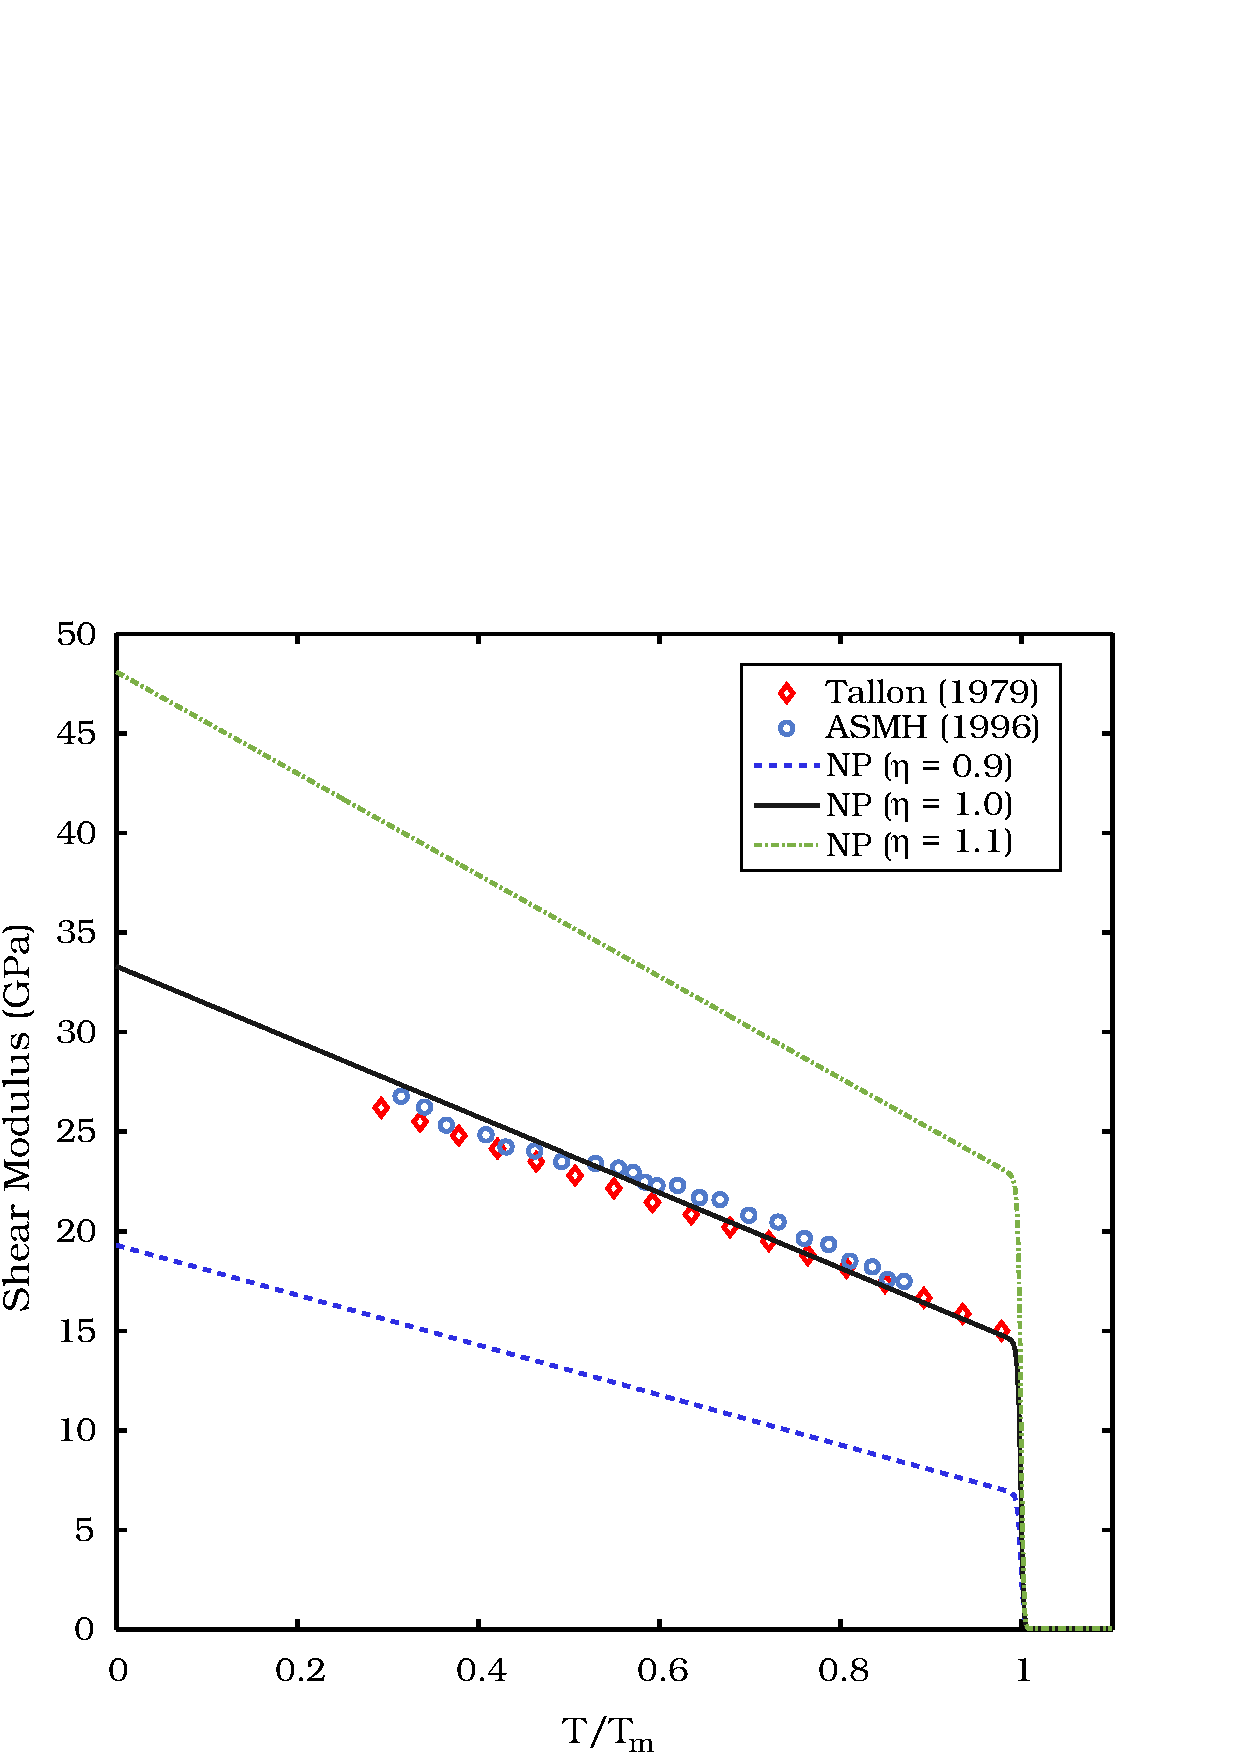
\includegraphics{FIGS/AlMuNP.pdf}} \\
          {\scriptsize Shear Modulus.}
        \end{column}
        \begin{column}{5cm}
          \centering
          \scalebox{0.30}{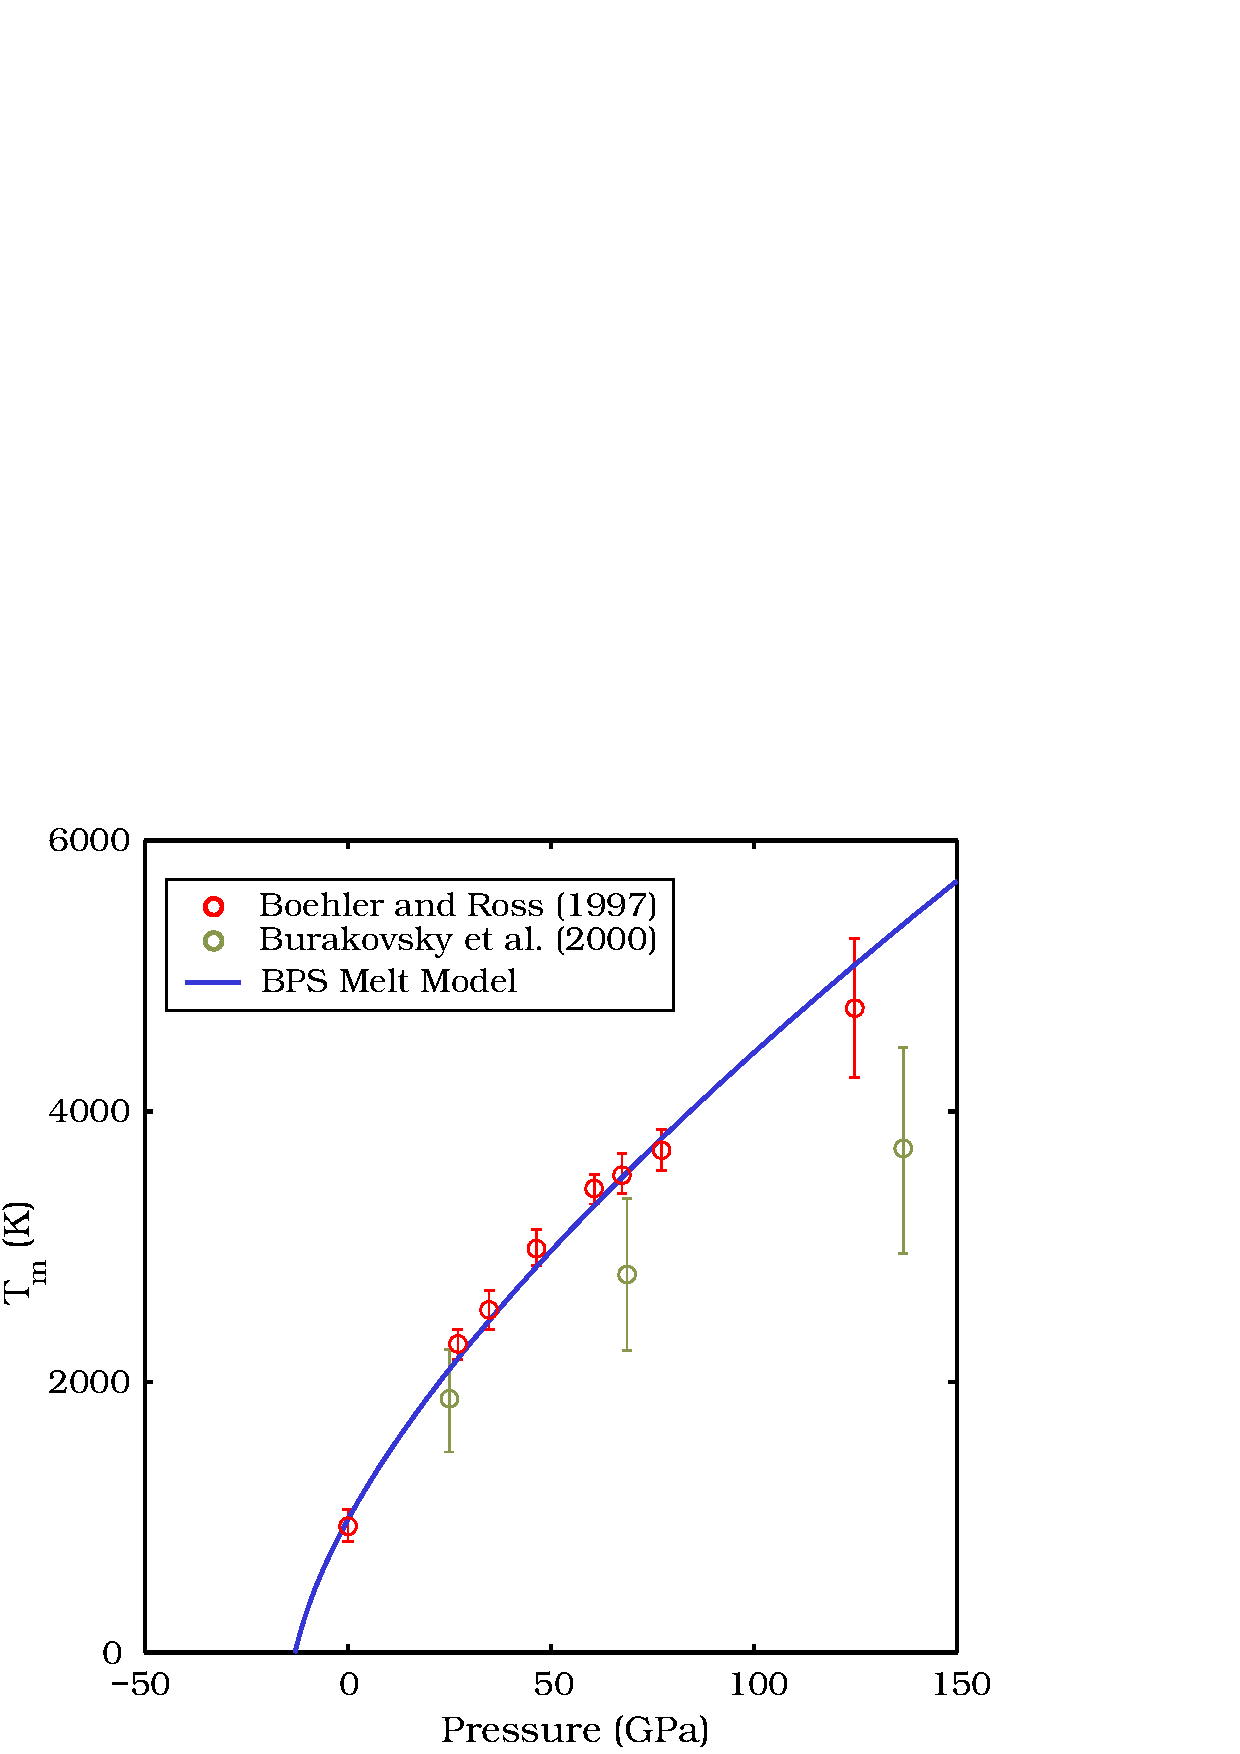
\includegraphics{FIGS/AlTm.pdf}} \\
          {\scriptsize Melt Temperature.}
        \end{column}
      \end{columns}
    \end{frame}

    \begin{frame}
      \frametitle{Model Validation: Flow Stress Model}
      \begin{columns}[t]
        \begin{column}{5cm}
          \centering
          \scalebox{0.26}{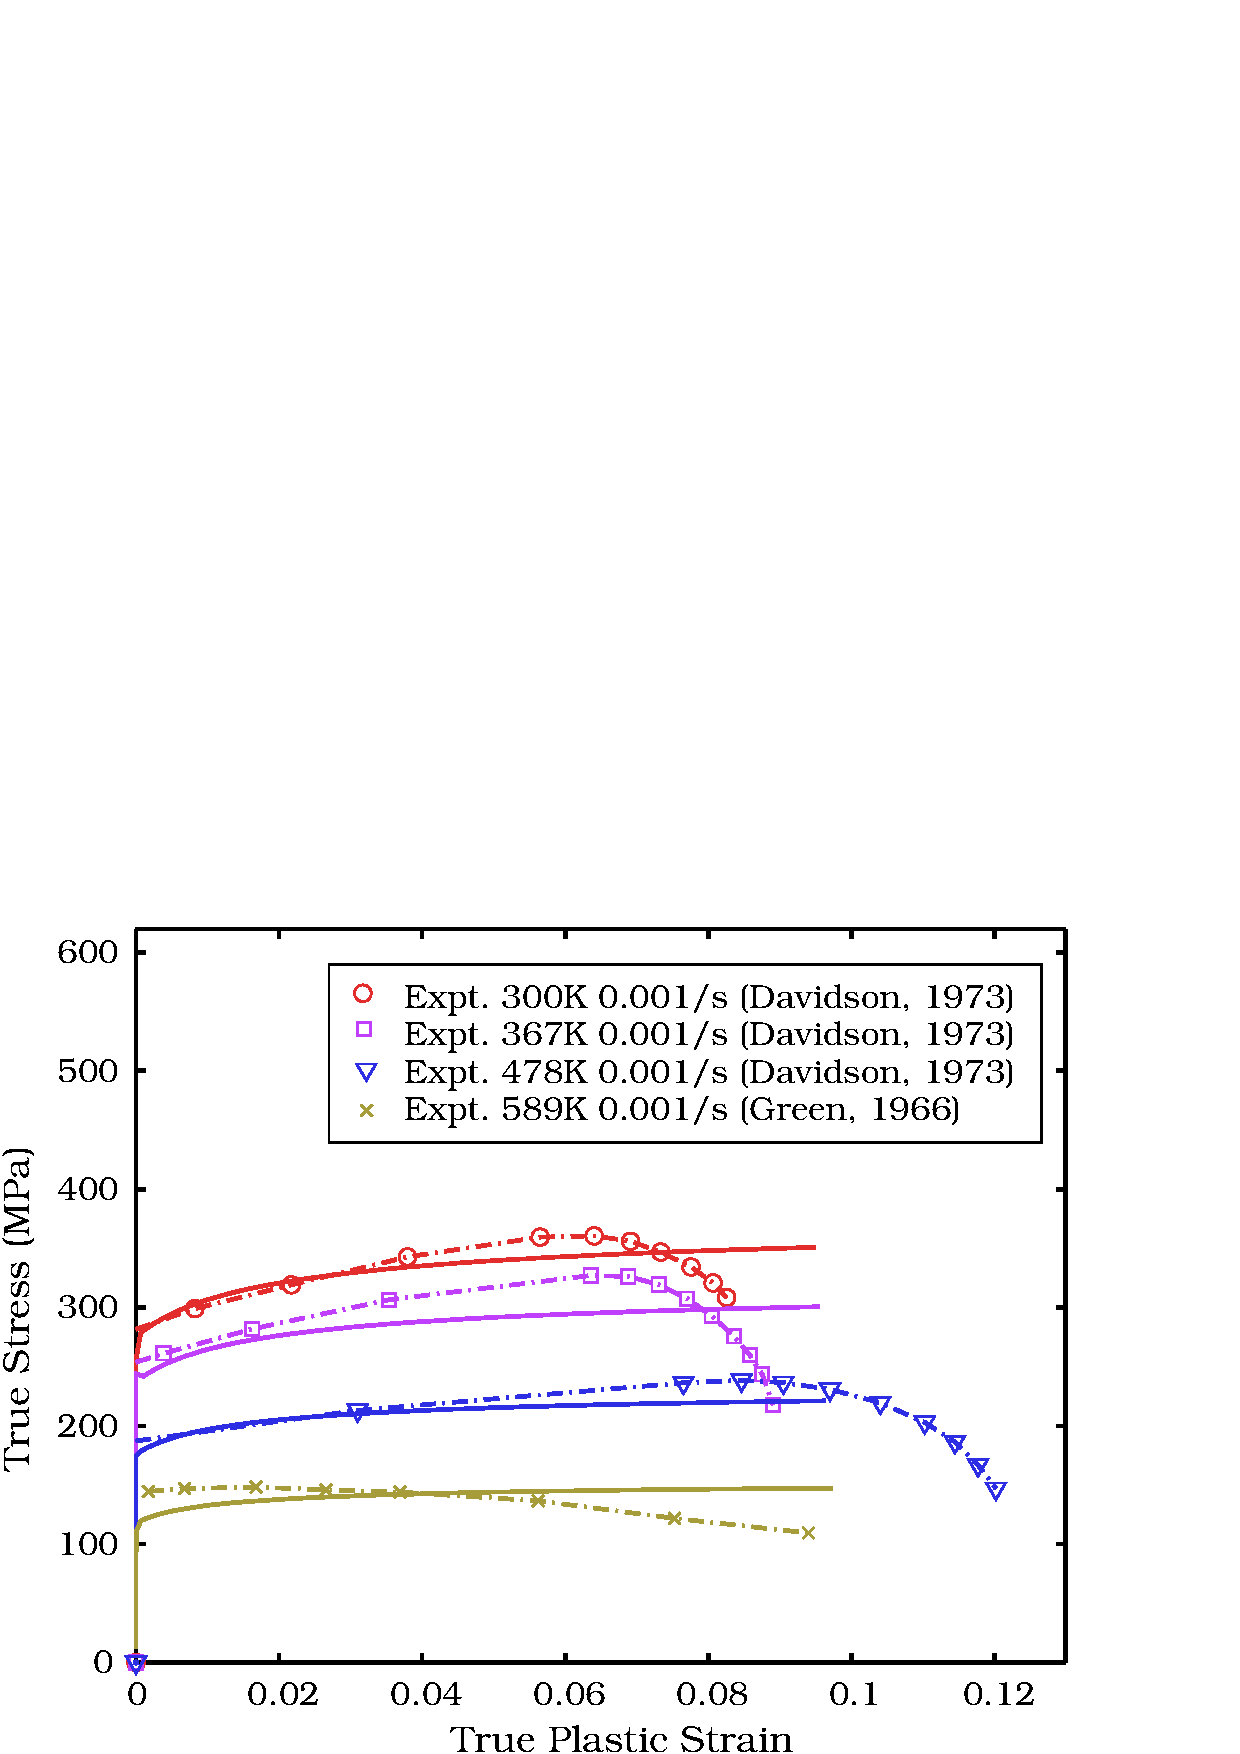
\includegraphics{FIGS/Al6061T6_0001s.pdf}} \\
          {\scriptsize Strain rate = 0.0001/s.}
        \end{column}
        \begin{column}{5cm}
          \centering
          \scalebox{0.26}{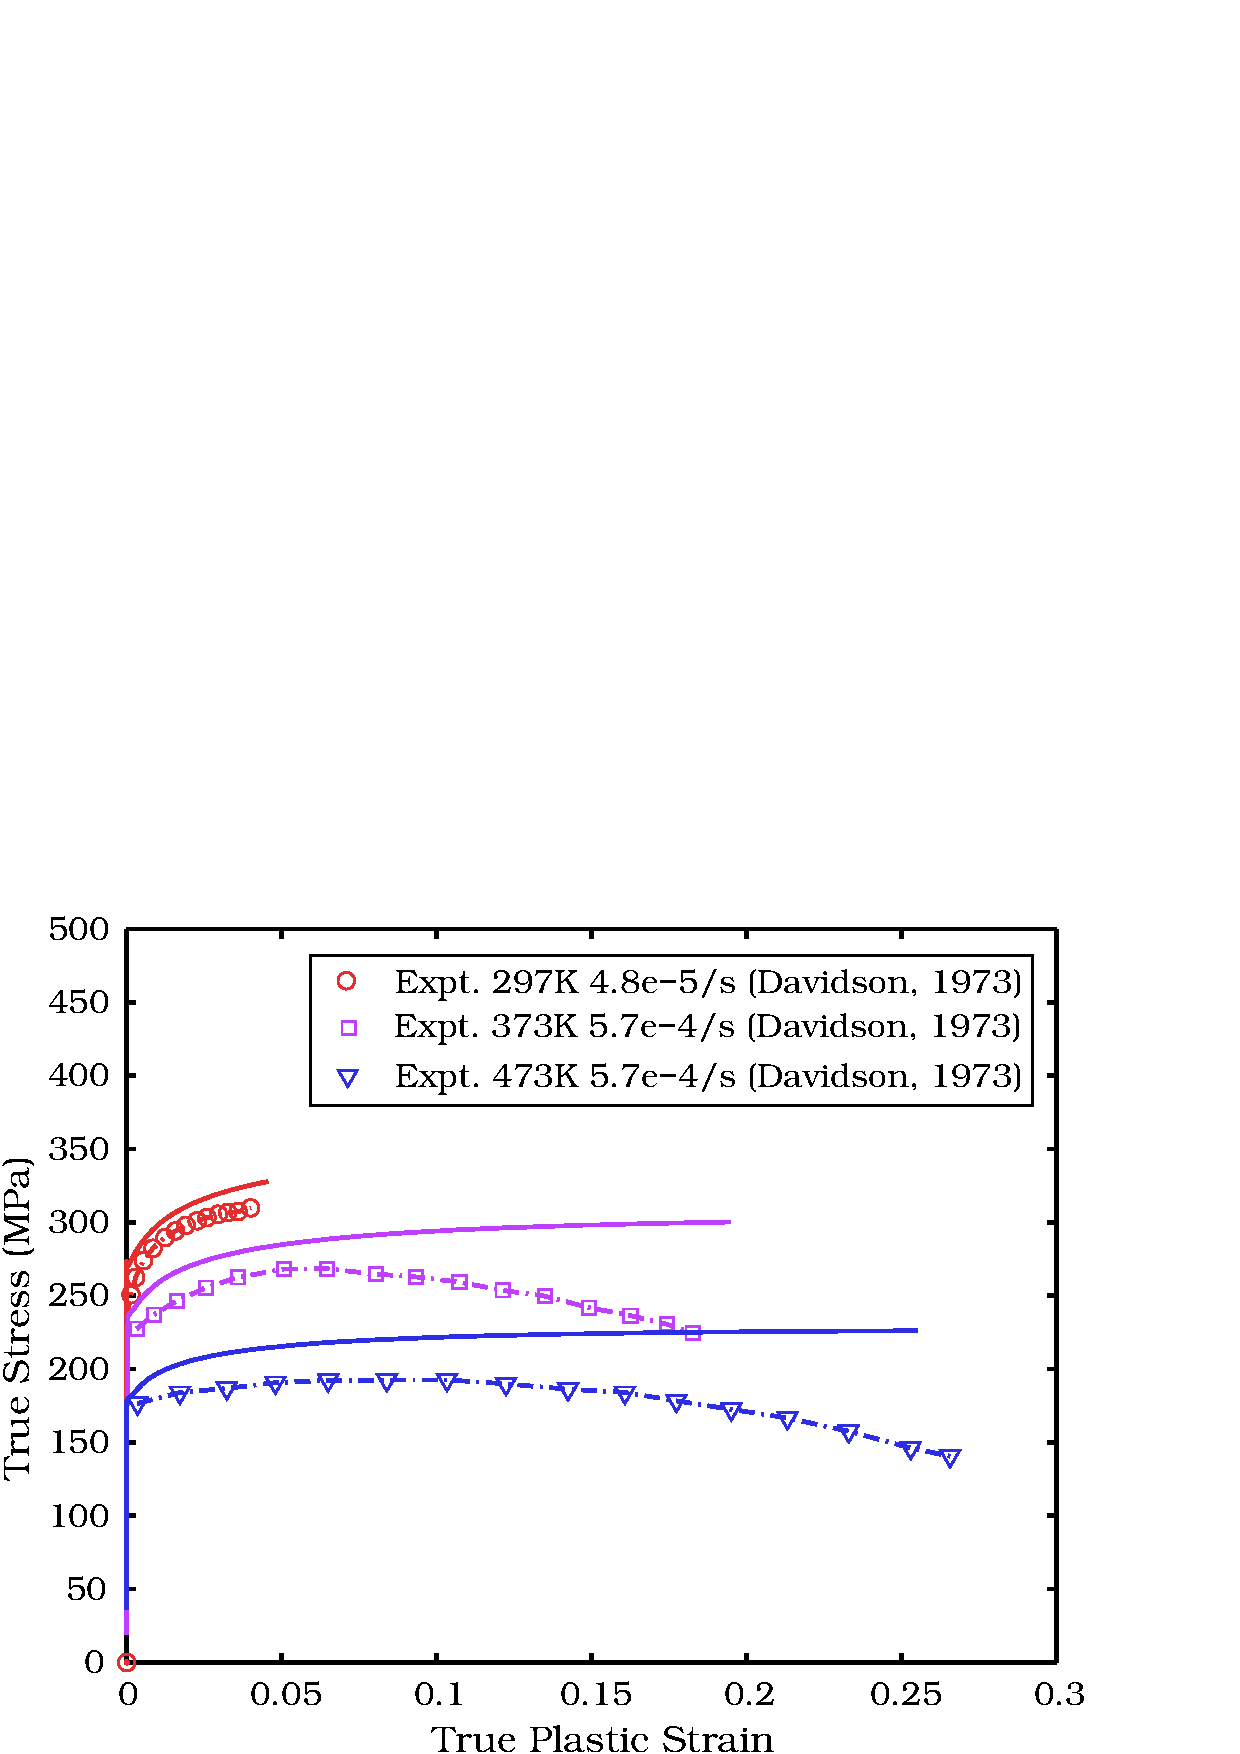
\includegraphics{FIGS/Al6061T6_0057s.pdf}} \\
          {\scriptsize Strain rate = 0.0057/s.}
        \end{column}
      \end{columns}
    \end{frame}

    \begin{frame}
      \frametitle{Model Validation: Flow Stress Model}
      \begin{columns}[c]
        \begin{column}{5cm}
          \centering
          \scalebox{0.20}{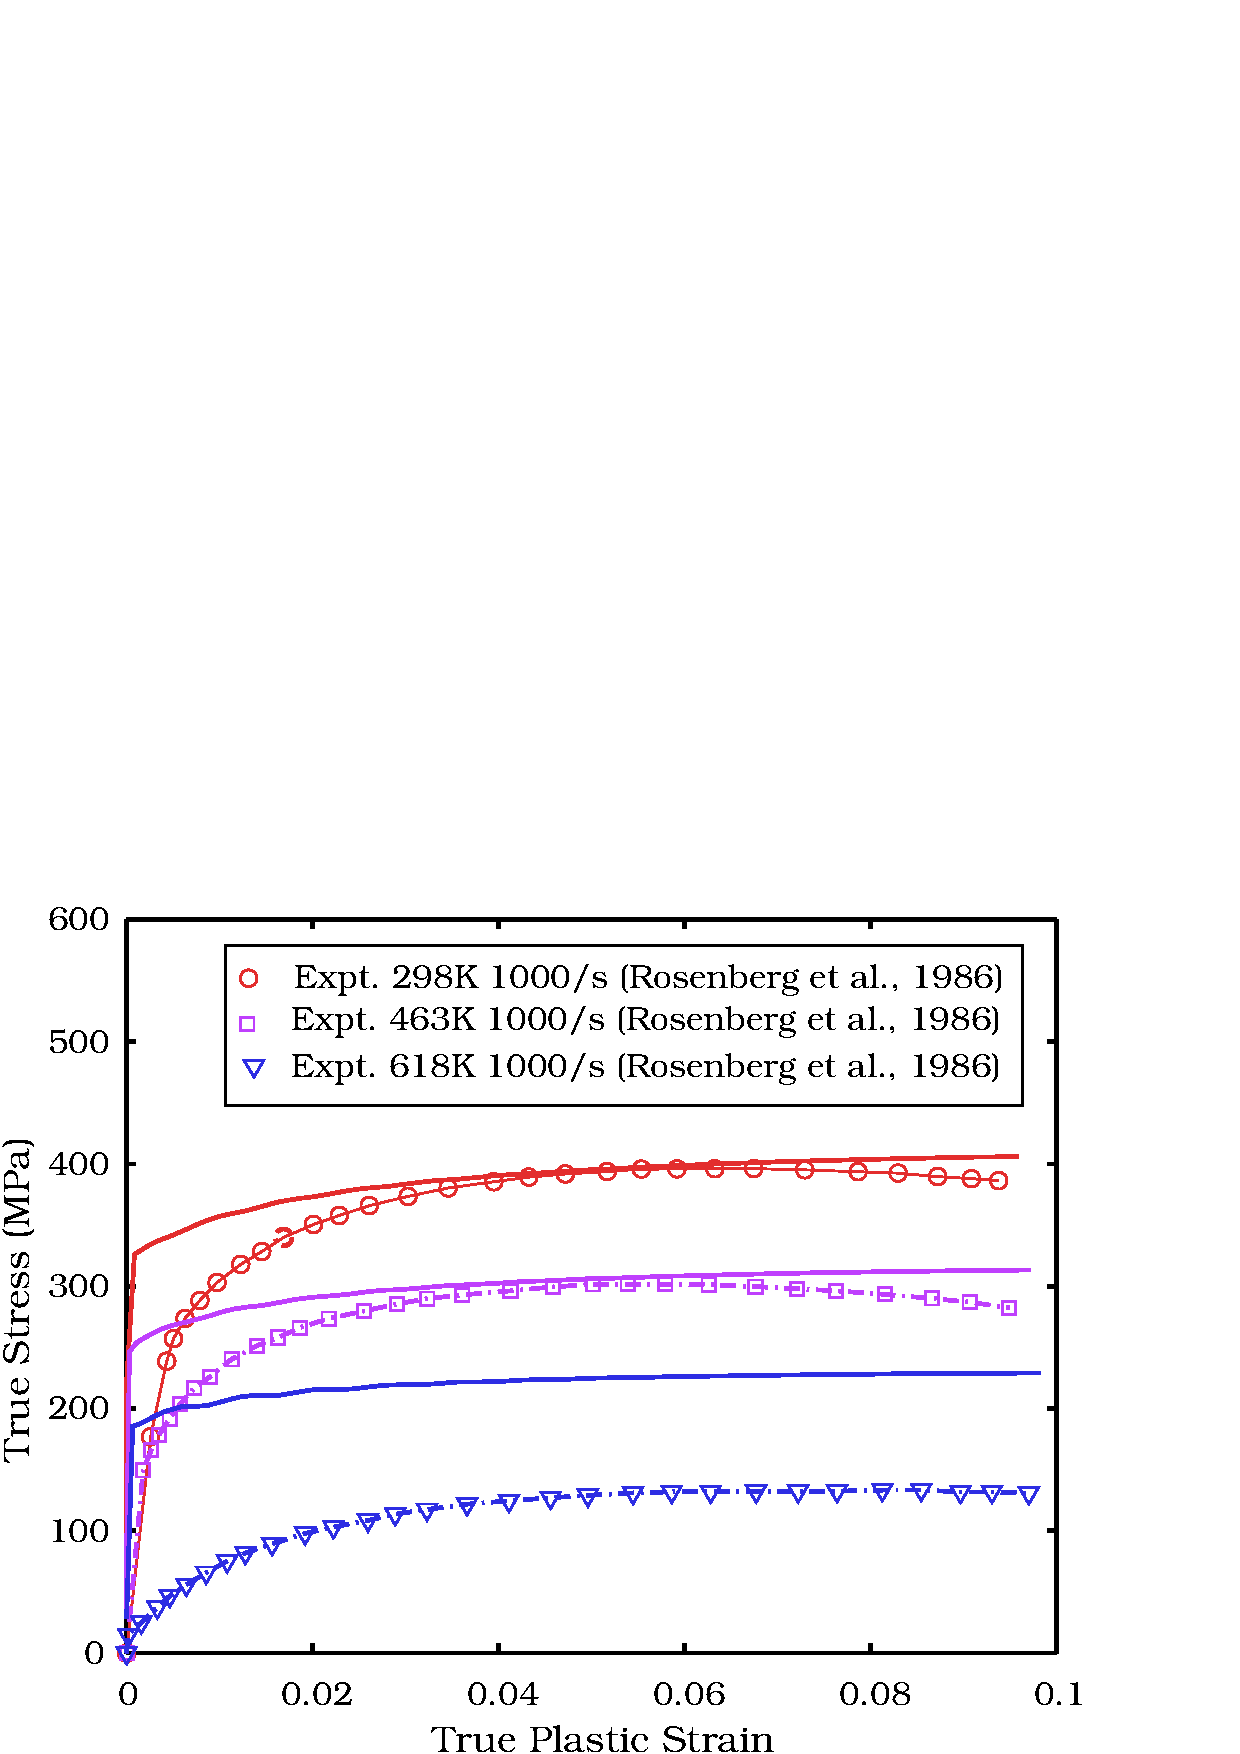
\includegraphics{FIGS/Al6061T6_1000s.pdf}} \\
          {\scriptsize Strain rate = 1000/s.}\\
          \vspace{12pt}
          \scalebox{0.20}{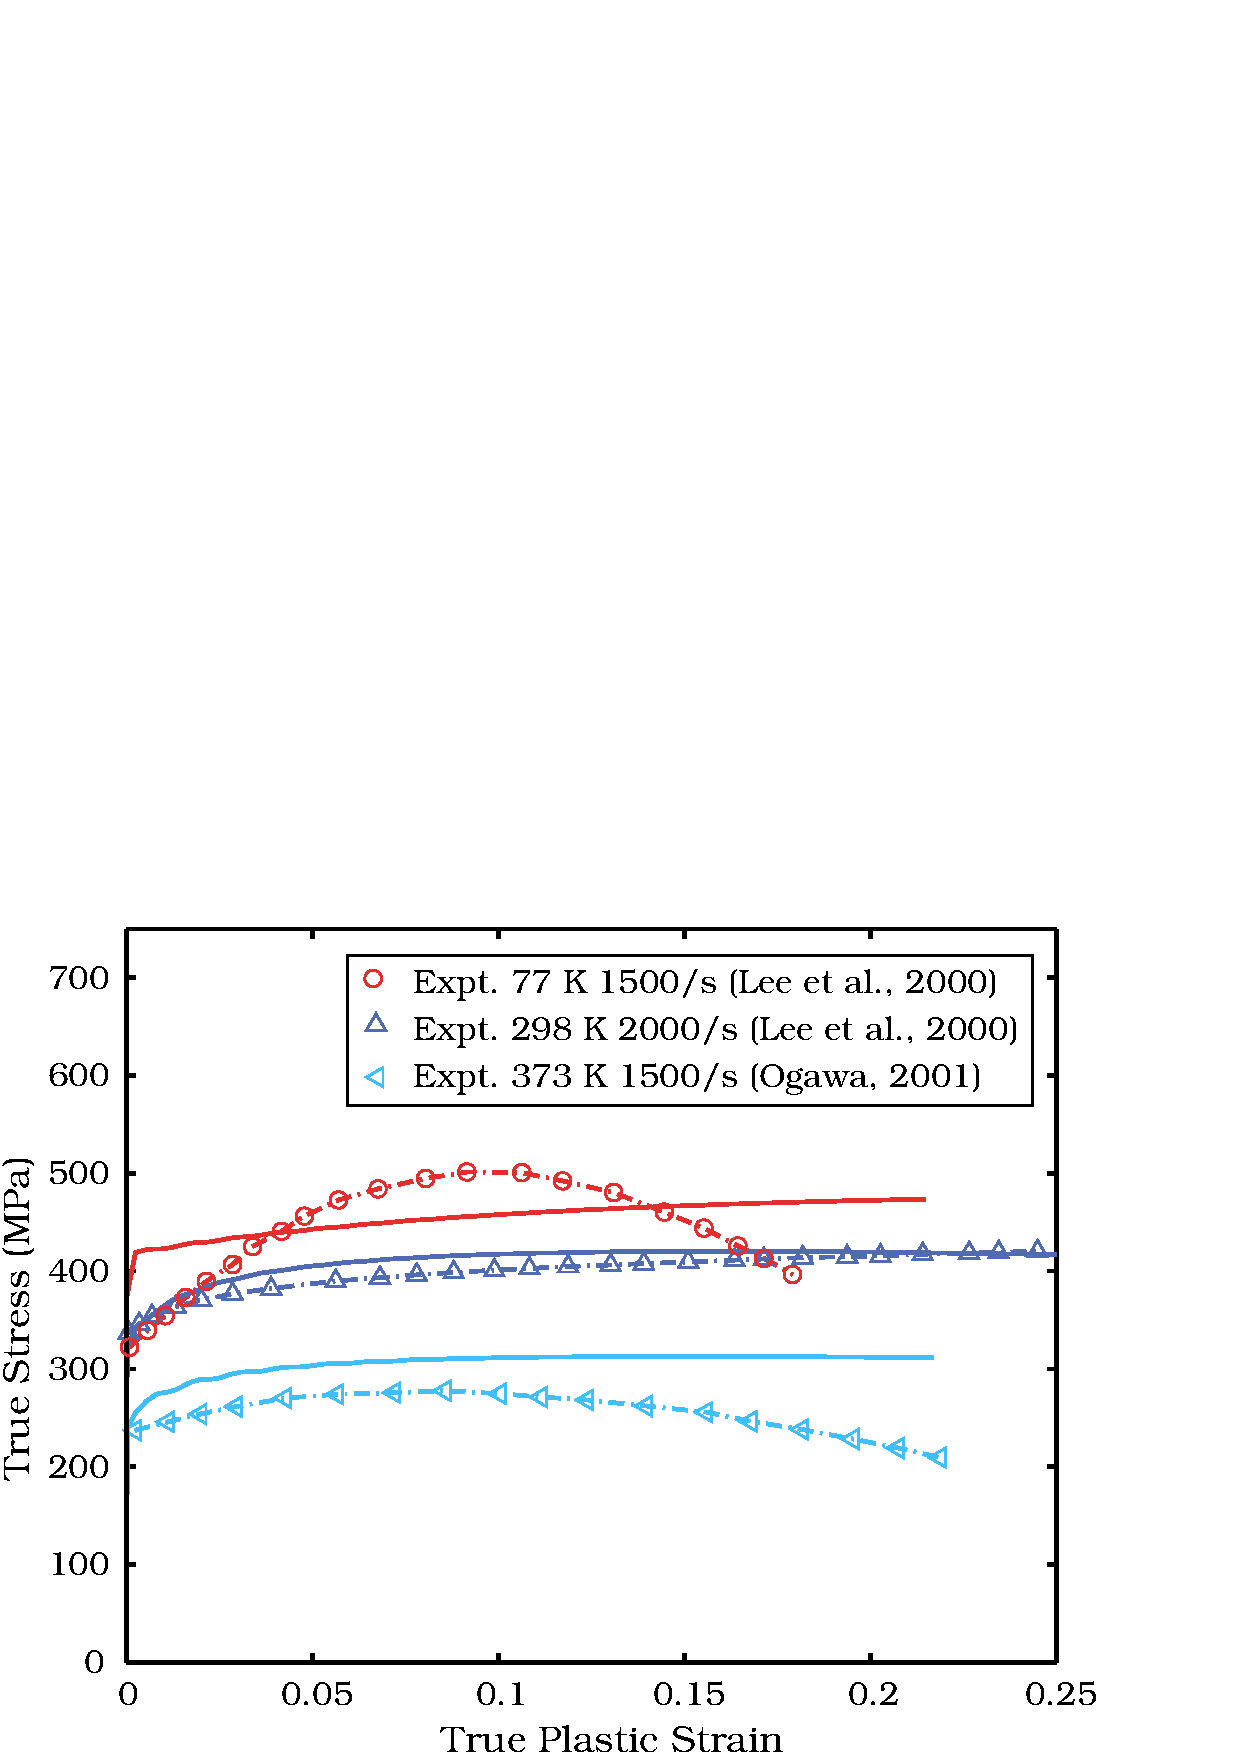
\includegraphics{FIGS/Al6061T6_2000s.pdf}} \\
          {\scriptsize Strain rate = 1500-2000/s.}
        \end{column}
        \begin{column}{5cm}
          \centering
          \scalebox{0.26}{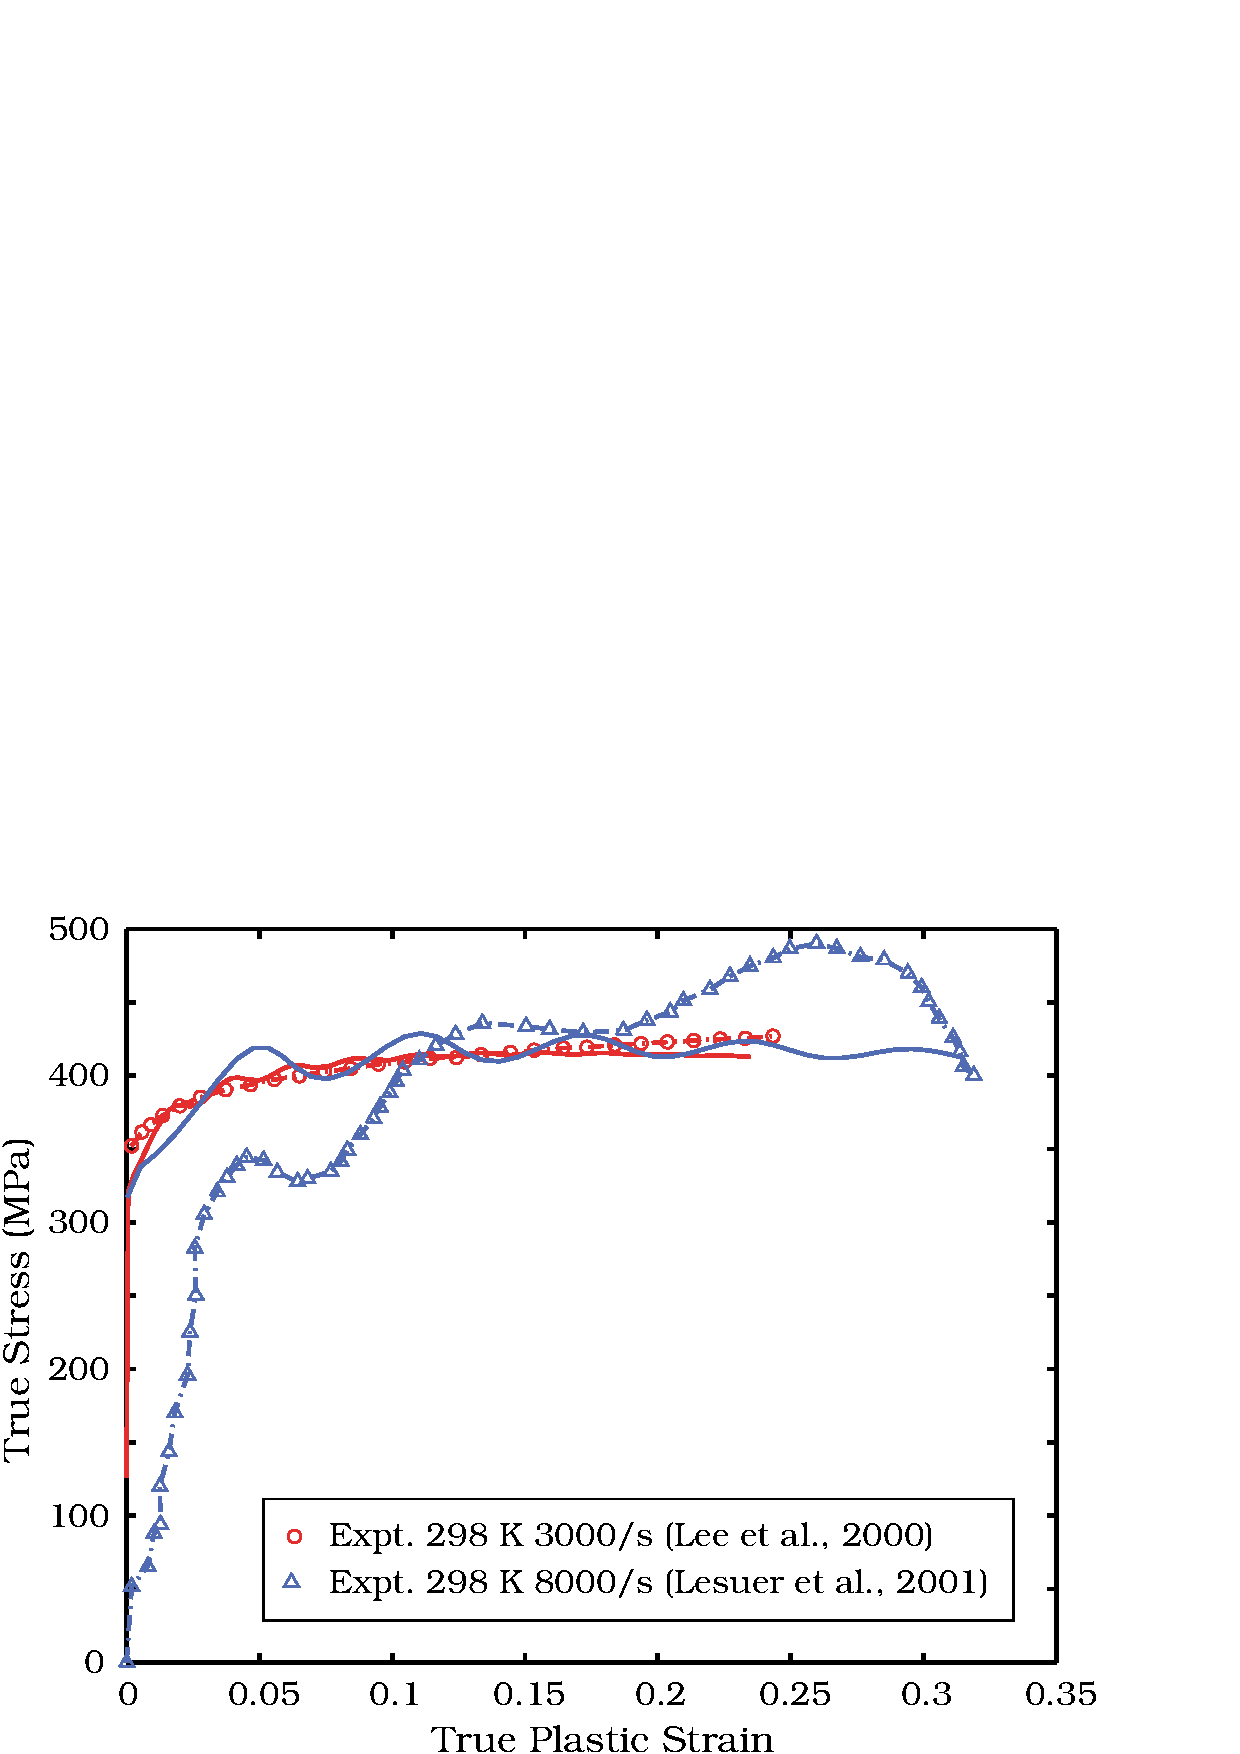
\includegraphics{FIGS/Al6061T6_3000-8000s.pdf}} \\
          {\scriptsize Strain rate = 3000-8000/s.}
        \end{column}
      \end{columns}
    \end{frame}

  \section{Creation of Foam Microstructures}

    \begin{frame}
      \frametitle{Bubble Creation}
      \begin{center}
        \centering
        \scalebox{0.20}{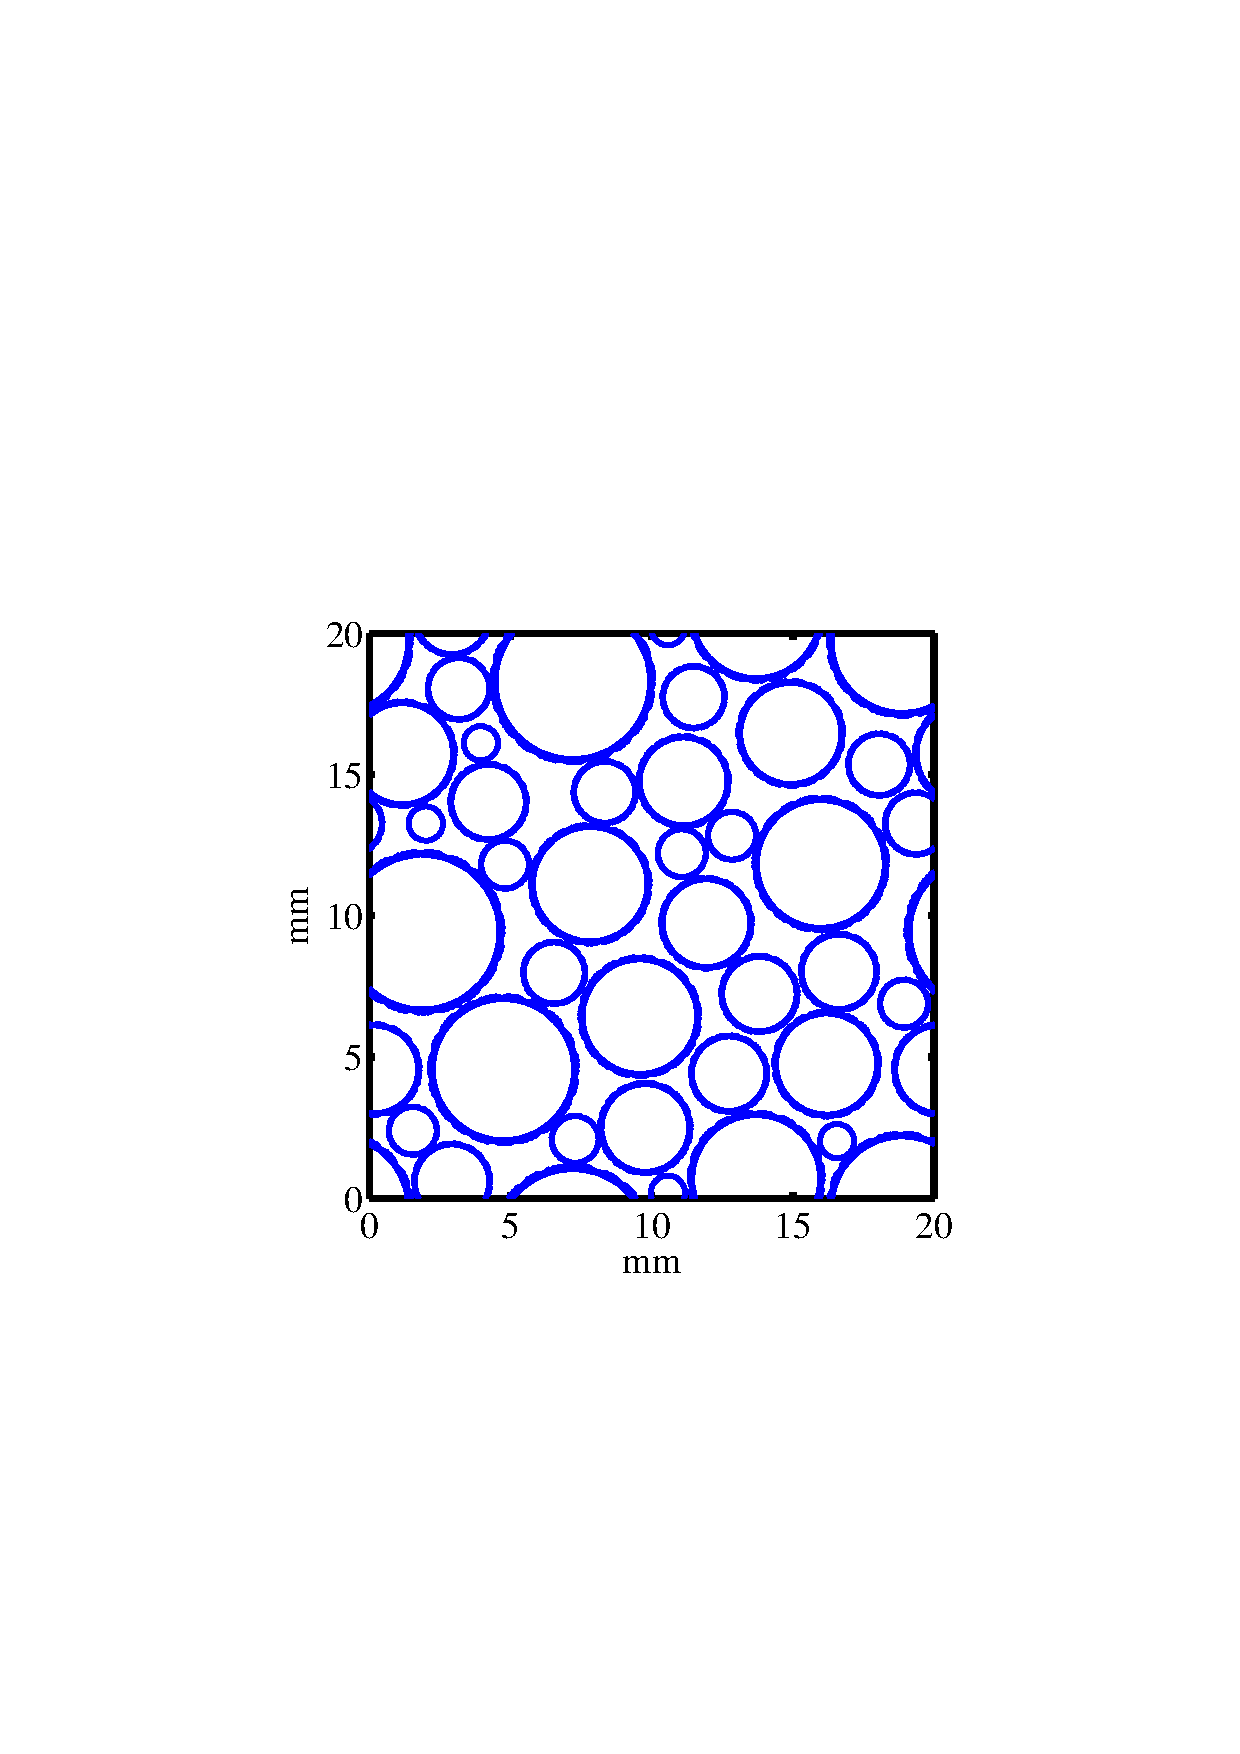
\includegraphics{FIGS/part_20mm.pdf}}
        \scalebox{0.20}{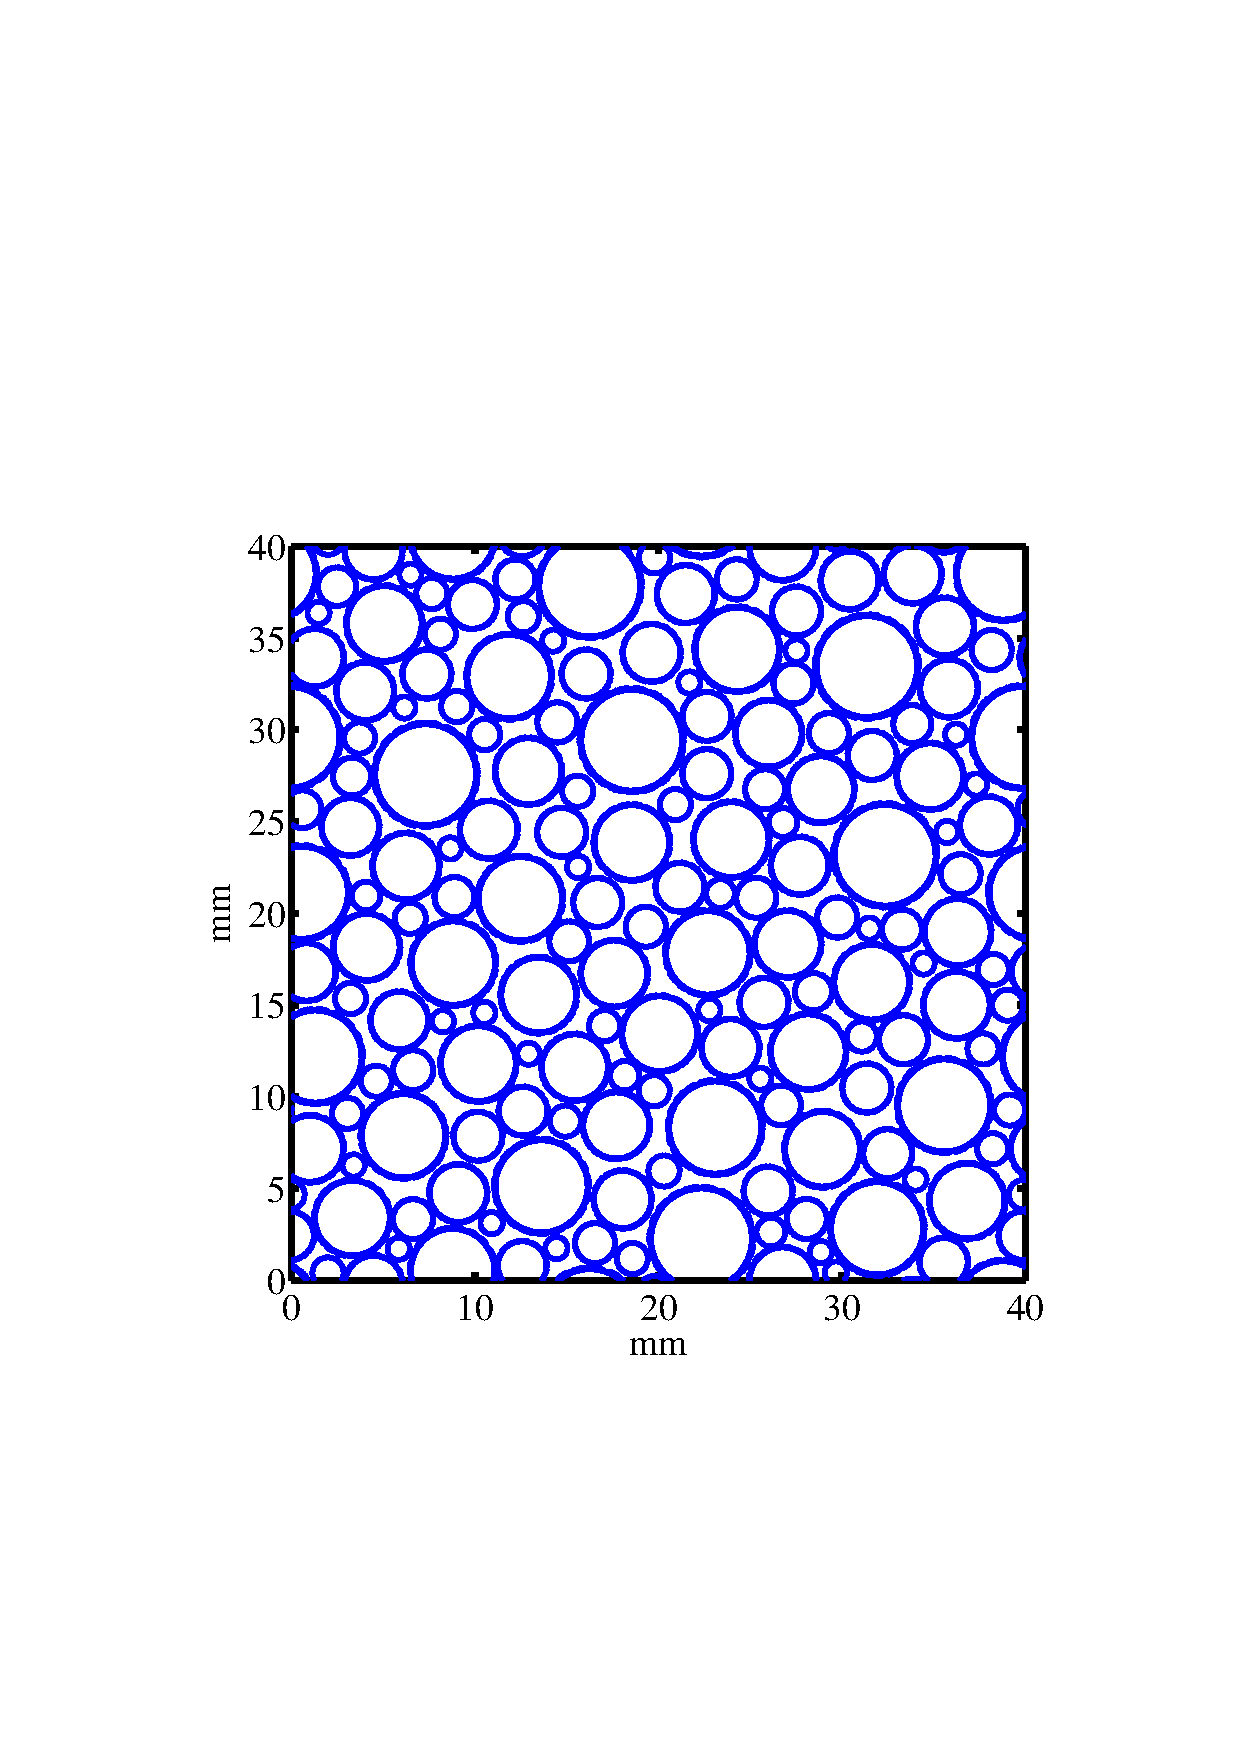
\includegraphics{FIGS/part_40mm.pdf}}
        \scalebox{0.26}{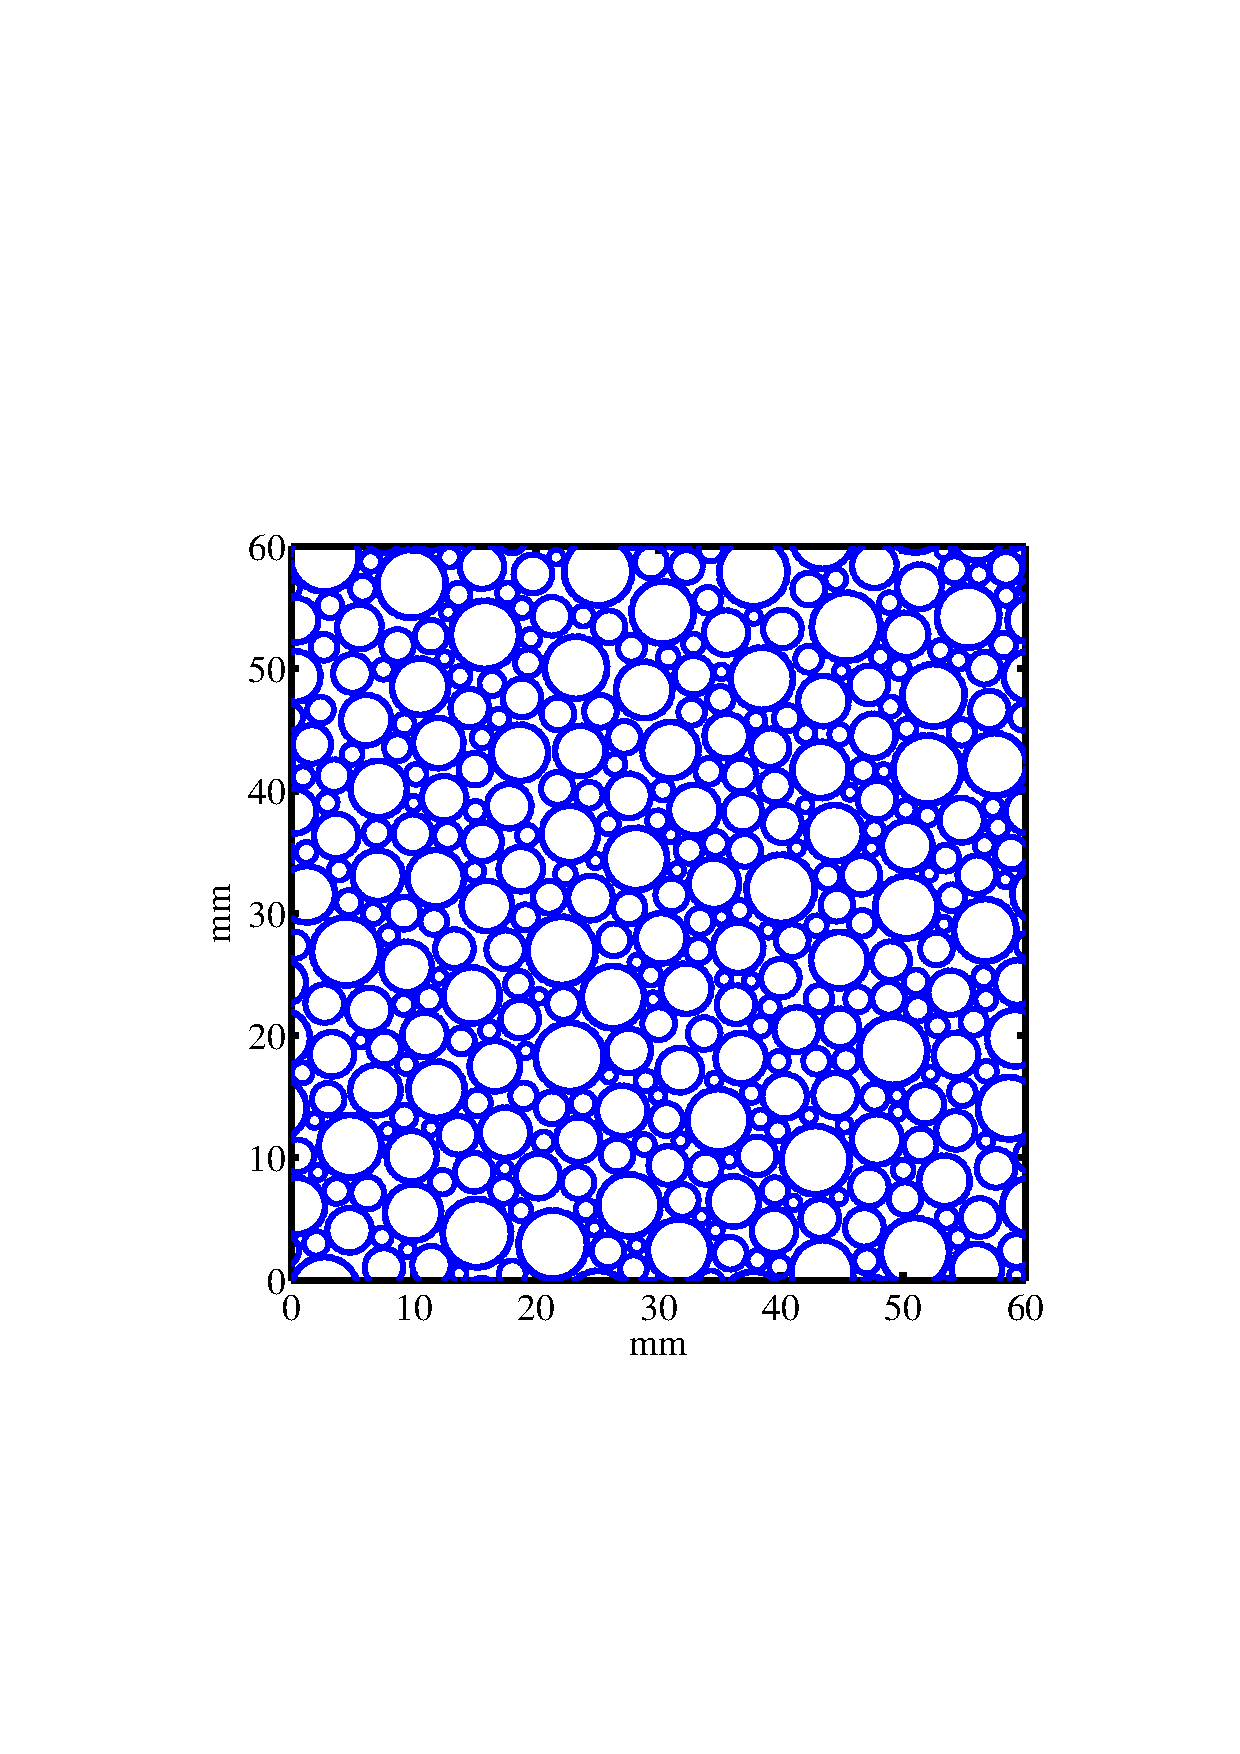
\includegraphics{FIGS/part_60mm.pdf}}
      \end{center}
      \begin{itemize}[<+-| alert@+>]
        \item Use a Poisson process to create bubble distribution.
        \item Periodic RVE.
        \item Uses input size distribution and volume fraction. 
      \end{itemize}
    \end{frame}

    \begin{frame}
      \frametitle{Bubble Pressurization}
      \scalebox{0.17}{\includegraphics{FIGS/foamCreate40mm_1.jpg}}
      \hspace{12pt}
      \scalebox{0.17}{\includegraphics{FIGS/foamCreate40mm_3.jpg}}
      \hspace{12pt}
      \scalebox{0.17}{\includegraphics{FIGS/foamCreate40mm_5.jpg}}
      \begin{itemize}[<+-| alert@+>]
        \item Use fluid-structure interaction to expand bubbles.
        \item Compressible Neo-Hookean solid with $K = $ 0.6 MPa and
              $\mu = $ 0.3 MPa.
        \item Gas inside bubbles is pressurized by adding heat.
        \item Gas between bubbles has low pressure and temperature.
      \end{itemize}
    \end{frame}

  \section{Crushing of Foam Microstructures}

    \begin{frame}
      \frametitle{Crushing Without Interior Gas}
      \scalebox{0.17}{\includegraphics{FIGS/foamCrush40mm_v1_ng_200ms_01.jpg}
                      \hspace{12pt}
                      \includegraphics{FIGS/foamCrush40mm_v1_ng_200ms_03.jpg}
                      \hspace{12pt}
                      \includegraphics{FIGS/foamCrush40mm_v1_ng_200ms_05.jpg}}\\
      \vspace{12pt}
      \scalebox{0.17}{\includegraphics{FIGS/foamCrush40mm_v1_ng_200ms_07.jpg}
                      \hspace{12pt}
                      \includegraphics{FIGS/foamCrush40mm_v1_ng_200ms_09.jpg}
                      \hspace{12pt}
                      \includegraphics{FIGS/foamCrush40mm_v1_ng_200ms_11.jpg}}
    \end{frame}

    \begin{frame}
      \frametitle{Crushing With Interior Gas}
      \scalebox{0.15}{\includegraphics{FIGS/foamCrush40mm_v1_g_200ms_01.jpg}
                      \hspace{12pt}
                      \includegraphics{FIGS/foamCrush40mm_v1_g_200ms_02.jpg}
                      \hspace{12pt}
                      \includegraphics{FIGS/foamCrush40mm_v1_g_200ms_03.jpg}}\\
      \vspace{12pt}
      \scalebox{0.15}{\includegraphics{FIGS/foamCrush40mm_v1_g_200ms_05.jpg}
                      \hspace{12pt}
                      \includegraphics{FIGS/foamCrush40mm_v1_g_200ms_07.jpg}
                      \hspace{12pt}
                      \includegraphics{FIGS/foamCrush40mm_v1_g_200ms_09.jpg}}
    \end{frame}

    \begin{frame}
      \frametitle{Stress-Strain Curves}
      \begin{center}
        \scalebox{0.35}{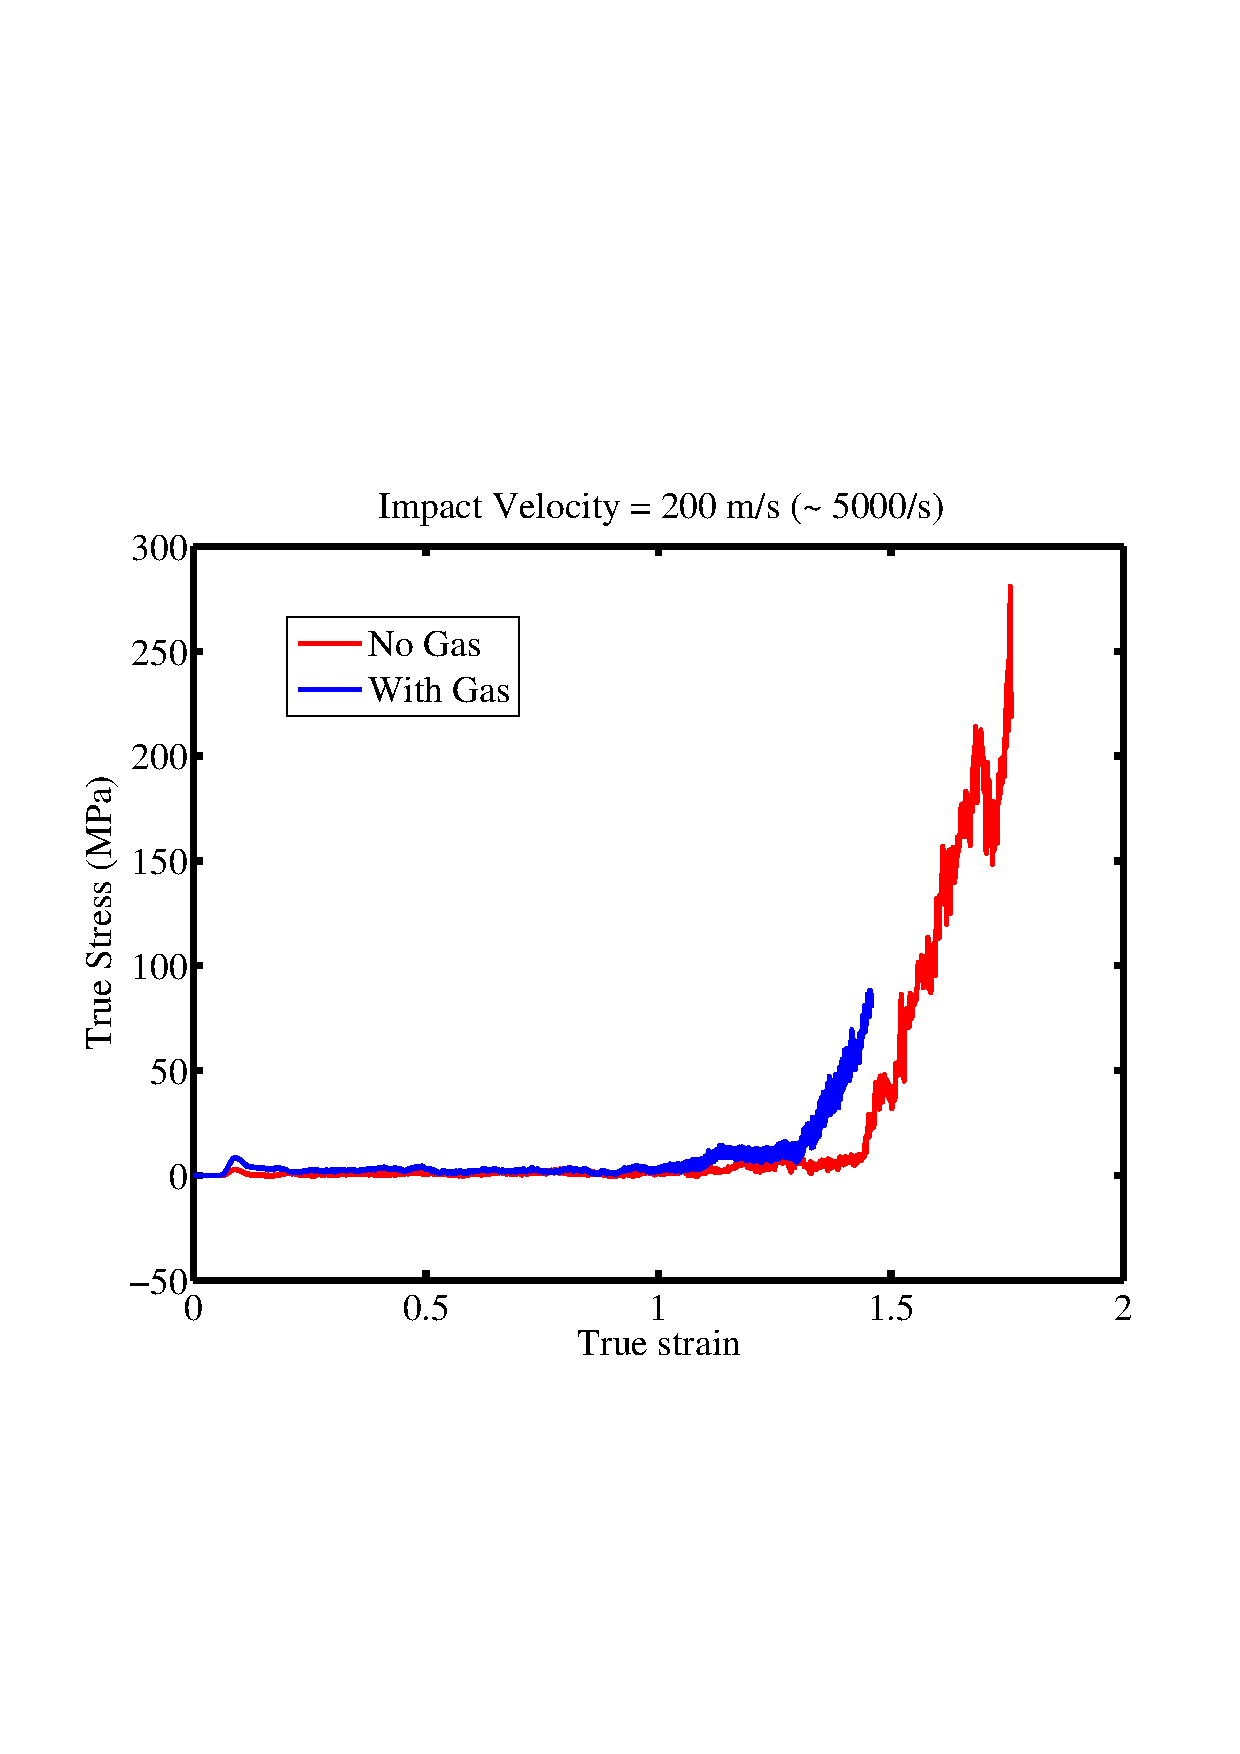
\includegraphics{FIGS/foamCrush40mm200msSigEps.pdf}} 
      \end{center}
    \end{frame}

    \begin{frame}
      \frametitle{Effect of Strain-Rate and Temperature}
      \begin{columns}[c]
        \begin{column}{5cm}
          \centering
          \scalebox{0.3}{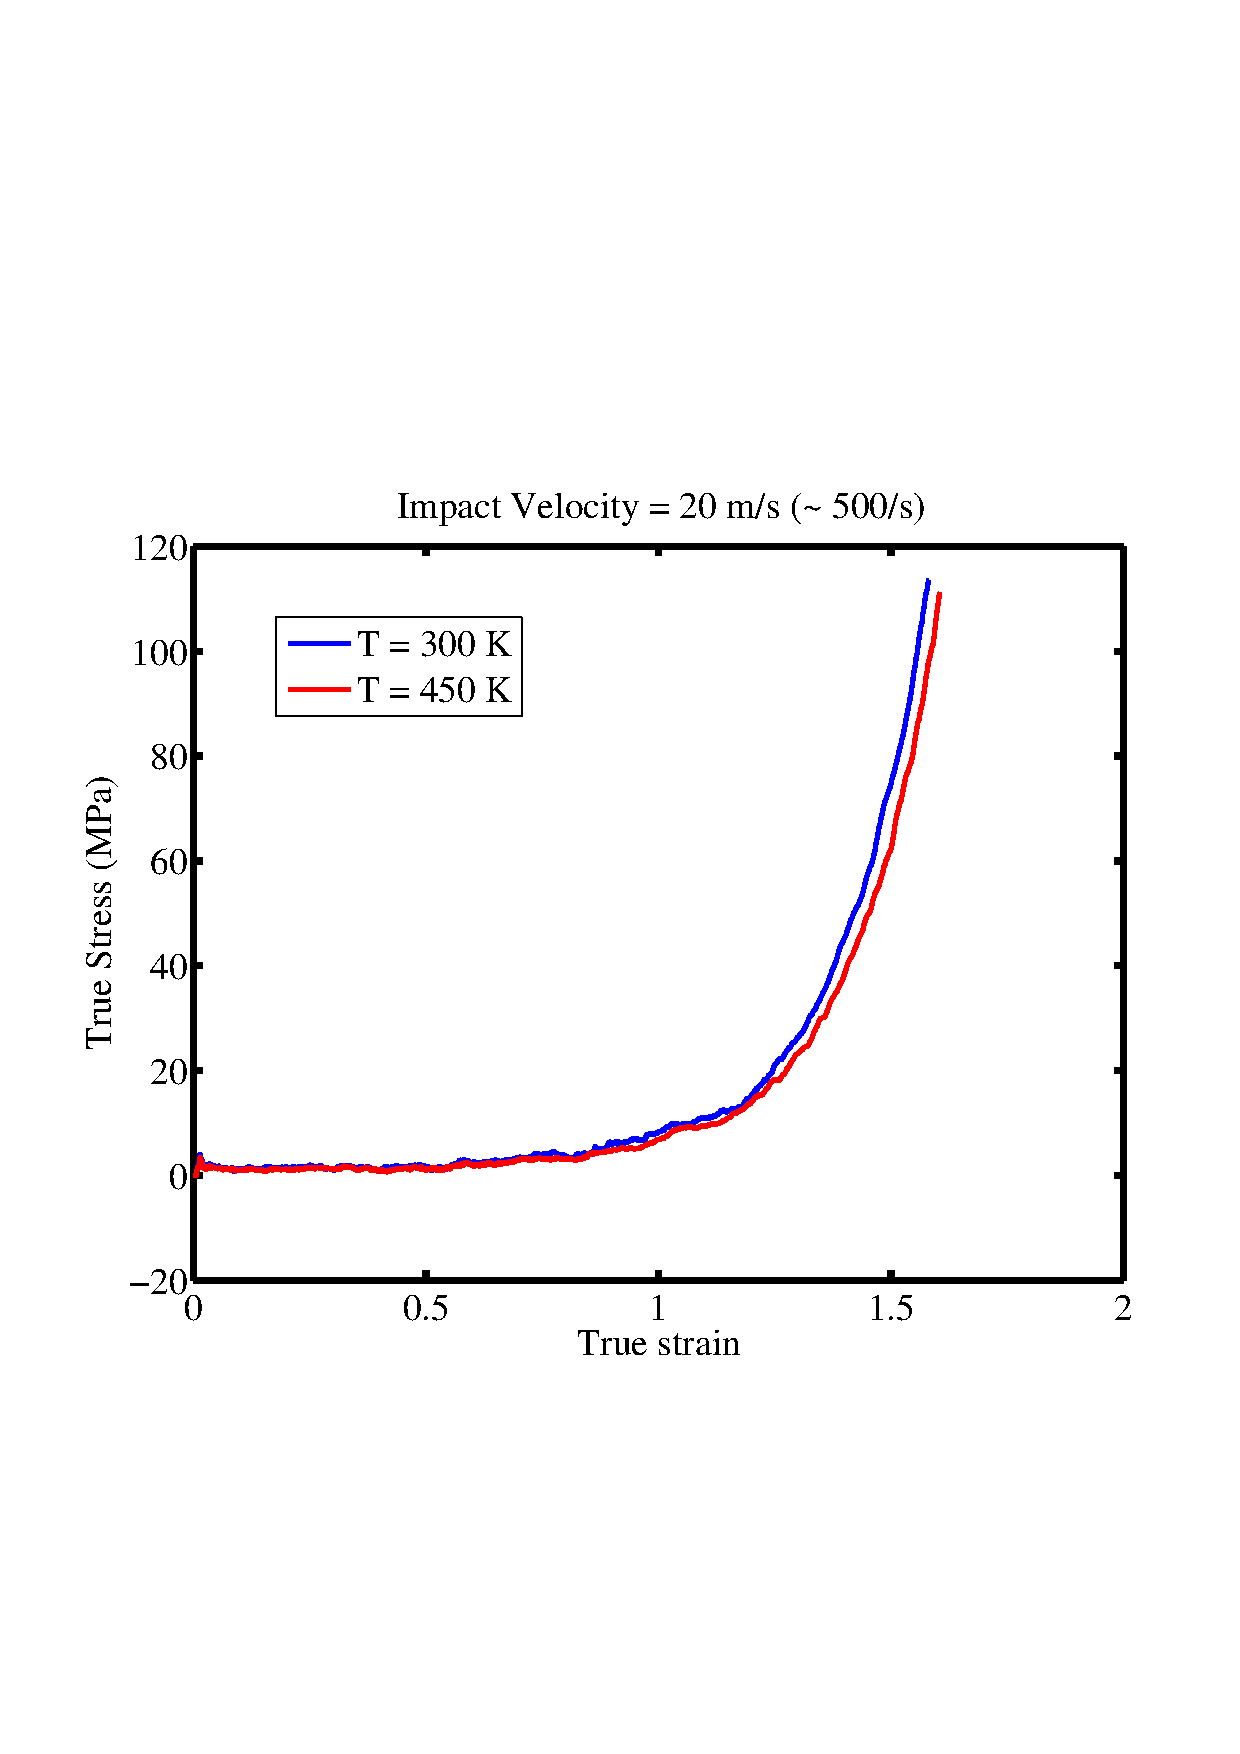
\includegraphics{FIGS/foamCrushSigEps_vel.pdf}} \\
          {\scriptsize Effect of Strain Rate}
        \end{column}
        \begin{column}{5cm}
          \centering
          \scalebox{0.3}{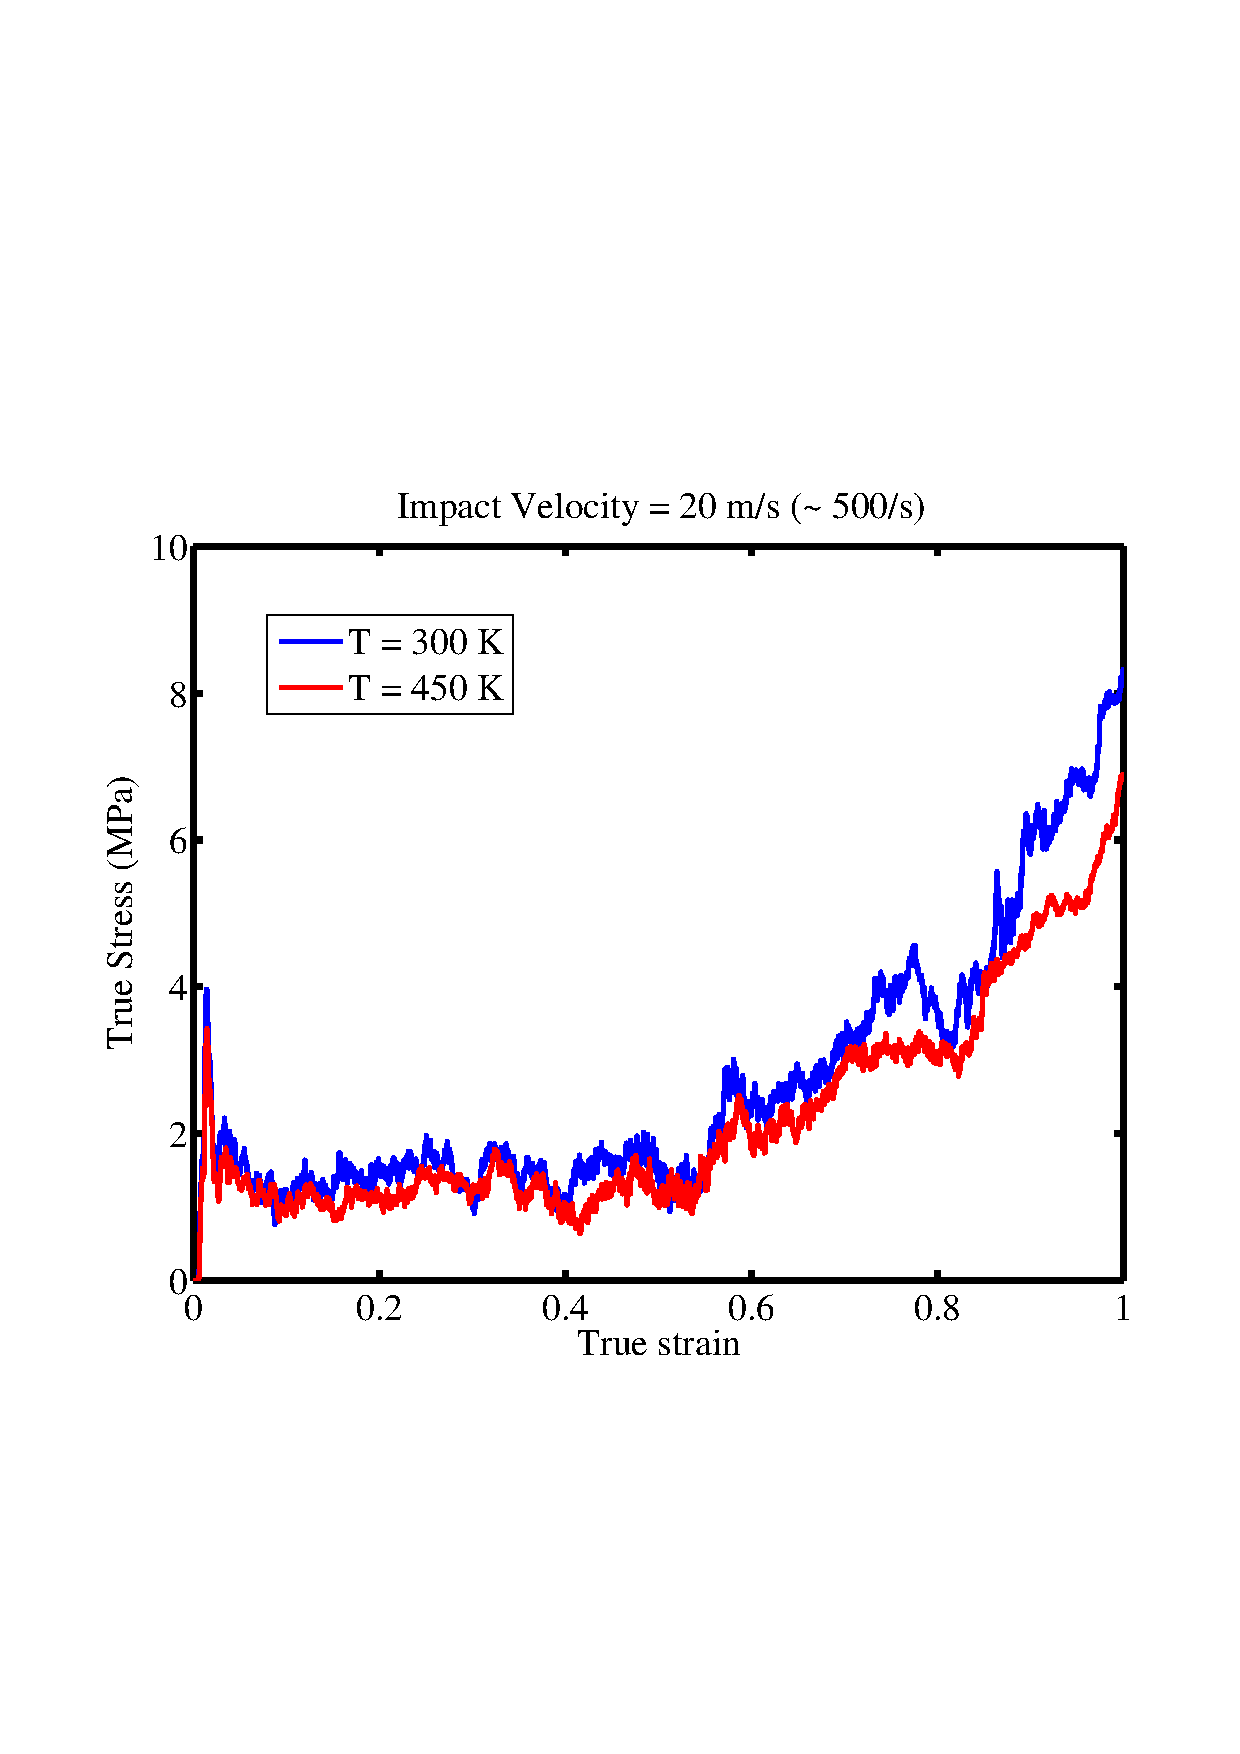
\includegraphics{FIGS/foamCrushSigEps_temp.pdf}} \\
          {\scriptsize Effect of Temperature}
        \end{column}
      \end{columns}
    \end{frame}
  \section*{Summary}

    \begin{frame}
      \frametitle<presentation>{Summary}
      \begin{itemize}
      \item
        MTS plasticity model of 6061-T6 Al.
      \item
        A novel way of creating a foam microstructure.
      \item 
        There is a clear effect of including gas in the
        stress-strain curves.
      \item
        Crushing of foam shows no shear banding. 
      \item
        Further work is needed to create a macroscopic 
        model of the dynamic response of Al foam.
      \end{itemize}
    \end{frame}

    \begin{frame}
      \frametitle{Creation of Foam Microstructure}
      \begin{center}
        \movie[loop,externalviewer]{\includegraphics[scale=0.25]{./FIGS/foamCreate40mm_4.jpg}}{foamCreate_40mm_v3_1.mpg}
      \end{center}
    \end{frame}

    \begin{frame}
      \frametitle{Crushing of Empty Foam}
      \begin{center}
        \movie[loop,externalviewer]{\includegraphics[scale=0.25]{./FIGS/foamCrush_ng.jpg}}{foamCrush40mm_ng_v1.mpg}
      \end{center}
    \end{frame}

    \begin{frame}
      \frametitle{Crushing of Gas-Filled Foam}
      \begin{center}
        \movie[loop,externalviewer]{\includegraphics[scale=0.25]{./FIGS/foamCrush.jpg}}{foamCrush40mm_v1_g.mpg}
      \end{center}
    \end{frame}


% All of the following is optional and typically not needed. 
%\appendix
%\section<presentation>*{\appendixname}
%\subsection<presentation>*{For Further Reading}
%
%\begin{frame}[allowframebreaks]
%  \frametitle<presentation>{For Further Reading}
%    
%  \begin{thebibliography}{10}
%    
%  \beamertemplatearticlebibitems
%  \bibitem{Banerjee06}
%    B.~Banerjee.
%    \newblock The mechanical threshold stress model for various
%                   tempers of 4340 steel.
%    \newblock {\em Int. J. Solids Struct.}, 2006, in press.
% 
%  \end{thebibliography}
%\end{frame}

\end{document}


